\documentclass[10pt, a4paper, twoside, openright]{report}

%packages-----------------------------------------------------------------------

\usepackage[utf8]{inputenc}
\usepackage[english]{babel}
\usepackage[T1]{fontenc}
\usepackage{lmodern}
\usepackage{array}
%\usepackage{times}
%\usepackage{helvet}
%\usepackage{charter}
\usepackage{graphicx}
\usepackage{color}
\usepackage{amsmath}
\usepackage{amssymb}
\usepackage{amsthm}
\usepackage{mathtools}
\usepackage{upgreek}
\usepackage{bm}
\usepackage{verbatim}
\usepackage{pdfpages}
\usepackage[unicode, pdfpagelayout=TwoPageRight]{hyperref}
\hypersetup{
	colorlinks=true,
	urlcolor=blue,
	linkcolor=blue,
	citecolor=blue
}
\newcommand{\link}[3][blue]{\href{#2}{\color{#1}{#3}}}%
\usepackage[small, bf]{caption}
\usepackage{enumerate}
\usepackage{epstopdf}
\usepackage{epsfig}
\usepackage{setspace}
\usepackage{diffcoeff}
\usepackage{enumitem}
\usepackage[inner=4.0cm, outer=3.0cm]{geometry}
\usepackage{emptypage}
\usepackage{caption}
%\usepackage{subcaption}
\usepackage{listings}
\usepackage{multicol}
\usepackage{multirow}
\usepackage{lipsum}
\usepackage{mathabx}
\usepackage{floatrow}
\usepackage{courier}
\usepackage{cite}
\def\citepunct{; \penalty\citepunctpenalty}
\usepackage[position=top]{subfig}
%\usepackage[autostyle]{csquotes}
\usepackage{microtype}

%\renewcommand{\familydefault}{\sfdefault}



\newcommand{\q}[1]{``#1''} % quotation marks

%cite----------



%fancystyles--------------------------------------------------------------------

\usepackage{fancyhdr}

\fancypagestyle{myfancy}{

\fancyhead[LE]{\nouppercase{\leftmark}}
\fancyhead[LO]{}
\fancyhead[CO]{}
\fancyhead[CE]{}
\fancyhead[RE]{}
\fancyhead[RO]{\nouppercase{\rightmark}}

\fancyfoot[LE]{\thepage}
\fancyfoot[LO]{}
\fancyfoot[CO]{}
\fancyfoot[CE]{}
\fancyfoot[RE]{}
\fancyfoot[RO]{\thepage}

\renewcommand{\headrulewidth}{0.4pt}
\renewcommand{\footrulewidth}{0.0pt}
}

\fancypagestyle{plain}{

\fancyhead[LE]{}
\fancyhead[LO]{}
\fancyhead[CO]{}
\fancyhead[CE]{}
\fancyhead[RE]{}
\fancyhead[RO]{}

\fancyfoot[LE]{\thepage}
\fancyfoot[LO]{}
\fancyfoot[CO]{}
\fancyfoot[CE]{}
\fancyfoot[RE]{}
\fancyfoot[RO]{\thepage}

\renewcommand{\headrulewidth}{0.0pt}
\renewcommand{\footrulewidth}{0.0pt}
}

%tikz---------------------------------------------------------------------------

\usepackage{tikz}
\usetikzlibrary{shapes, arrows}

%url----------------------------------------------------------------------------

\usepackage{url}
\DeclareUrlCommand\url{\def\UrlLeft{<}\def\UrlRight{>} \urlstyle{tt}}

%color--------------------------------------------------------------------------

\definecolor{darkred}{rgb}{0.6,0,0}
\definecolor{darkgreen}{rgb}{0,0.6,0}
\definecolor{darkblue}{rgb}{0,0,0.6}
\definecolor{darkgrey}{rgb}{0.3,0.3,0.3}
\definecolor{grey}{rgb}{0.6,0.6,0.6}
\definecolor{lightgrey}{rgb}{0.95,0.95,0.95}
\definecolor{lightred}{rgb}{0.99,0.85,0.85}
\definecolor{violet}{rgb}{0.65,0.45,0.75}

%listings-----------------------------------------------------------------------

\definecolor{mygreen}{rgb}{0,0.6,0}
\definecolor{mygray}{rgb}{0.5,0.5,0.5}
\definecolor{light}{rgb}{0.96, 0.96, 0.96}
\definecolor{mymauve}{rgb}{0.58,0,0.82}

\lstdefinestyle{CXX} {
	language=C++,
	backgroundcolor=\color{light},
	basicstyle=\scriptsize\ttfamily,
	breakatwhitespace=false,
	breaklines=true,
	captionpos=t,
	%commentstyle=\color{mygreen},
	deletekeywords={},
	escapeinside={\%*}{*)},
	extendedchars=true,
	frame=single,
	keepspaces=true,
	keywordstyle=\color{blue},
	otherkeywords={},
	numbers=left,
	numbersep=5pt,
	numberstyle=\tiny\color{mygray},
	rulecolor=\color{black},
	showspaces=false,
	showstringspaces=false, 
	showtabs=false,
	stepnumber=1,
	stringstyle=\color{mymauve},
	tabsize=3,
	title=\lstname   
}

\lstdefinestyle{FORTRAN} {
	language=[90]Fortran,
	backgroundcolor=\color{light},
	basicstyle=\scriptsize\ttfamily,
	keywordstyle=\color{blue},
	%commentstyle=\color{mygreen},
	breakatwhitespace=false,
	breaklines=true,
	captionpos=t,
	deletekeywords={},
	escapeinside={\%*}{*)},
	extendedchars=true,
	frame=single,
	keepspaces=true,
	otherkeywords={},
	numbers=left,
	numbersep=5pt,
	numberstyle=\tiny\color{mygray},
	rulecolor=\color{black},
	showspaces=false,
	showstringspaces=false, 
	showtabs=false,
	stepnumber=1,
	stringstyle=\color{mymauve},
	tabsize=3,
	title=\lstname 
}

%settings-----------------------------------------------------------------------

\setlength{\parindent}{15pt}
\setlength{\parskip}{0pt}
\renewcommand{\baselinestretch}{1.0}
\pagenumbering{arabic}
\frenchspacing

\DeclareFontFamily{U}{mathx}{\hyphenchar\font45}
\DeclareFontShape{U}{mathx}{m}{n}{<-> mathx10}{}
\DeclareSymbolFont{mathx}{U}{mathx}{m}{n}
\DeclareMathAccent{\widebar}{0}{mathx}{"73}

%commands----------------------------------------------------------------------

\newcommand{\ctu}{Czech Technical University in Prague}
\newcommand{\fnspe}{Faculty of Nuclear Sciences and Physical Engineering}
\newcommand{\dpe}{Department of Physical Electronics}
\newcommand{\branch}{Computational Physics}
\newcommand{\projecttitle}{Laser-driven sources of~electrons and~x-rays in~underdense plasma: Theory and~simulation}
\newcommand{\projecttitlecz}{Laserem řízené zdroje elektronů a~rentgenového záření v~podkritickém plazmatu: Teorie a~simulace}
\newcommand{\valenta}{Ing. Petr Valenta}
\newcommand{\klimo}{doc. Ing. Ondřej Klimo, Ph.D.}
\newcommand{\bulanov}{Prof. Sergei Vladimirovich Bulanov}
%\newcommand{\year}{2022}
%\newcommand{\keywords}{}
%\newcommand{\keywordscz}{}

%macros-------------------------------------------------------------------------

\newcommand{\nucl}[3]{
\ensuremath{
\phantom{
\ensuremath{^{#1}_{#2}}}
\llap{\ensuremath{^{\rule{0pt}{0pt}#1}}}
\llap{\ensuremath{_{\rule{0pt}{7pt}#2}}}
\mbox{#3}}}

\newcommand{\norm}[1]{\lVert#1\rVert}
\newcommand{\abs}[1]{\lvert#1\rvert}

\renewcommand{\vec}[1]{\boldsymbol{\mathrm{#1}}}

\newcommand{\rot}[1]{\nabla \times #1}
\newcommand{\grad}[1]{\nabla #1}
\renewcommand{\div}[1]{\nabla \cdot #1}
\newcommand{\laplace}[1]{\Delta #1}
\newcommand{\dalembert}[1]{\Box #1}

\newcommand{\e}[0]{\mathrm{e}}
\renewcommand{\i}[0]{\mathrm{i}}
\renewcommand{\d}[0]{\mathrm{d}}

%changecountering---------------------------------------------------------------

\usepackage{chngcntr}
%\counterwithout{equation}{chapter}
\counterwithout{figure}{chapter}
\counterwithout{table}{chapter}

% quotes------------------------------------------------------------------------

\usepackage[newcentury, nogrey]{quotchap}
\makeatletter
\renewcommand*{\sectfont}{\bfseries}
\let\size@chapter\Huge
\renewcommand*{\chapnumfont}{%
	\usefont{T1}{\@defaultcnfont}{b}{n}\fontsize{130}{100}\selectfont% Default: 100/130
	\color{chaptergrey}%
}
\makeatother
\definecolor{chaptergrey}{rgb}{0.95, 0.95, 0.95}

% fancy quotes
\definecolor{quotemark}{rgb}{0.8, 0.8, 0.8}
\makeatletter
\def\fquote{%
	\@ifnextchar[{\fquote@i}{\fquote@i[]}%]
}%
\def\fquote@i[#1]{%
	\def\tempa{#1}%
	\@ifnextchar[{\fquote@ii}{\fquote@ii[]}%]
}%
\def\fquote@ii[#1]{%
	\def\tempb{#1}%
	\@ifnextchar[{\fquote@iii}{\fquote@iii[]}%]
}%
\def\fquote@iii[#1]{%
	\def\tempc{#1}%
	%\vspace{1em}%
	\noindent%
	\begin{list}{}{%
			\setlength{\leftmargin}{0.1\textwidth}%
			\setlength{\rightmargin}{0.1\textwidth}%
		}%
		\item[]%
		\begin{picture}(0,0)%
			\put(-15,-5){\makebox(0,0){\scalebox{3}{\textcolor{quotemark}{``}}}}%
		\end{picture}%
		\begingroup\itshape}%
	\def\endfquote{%
		\endgroup\par%
		\makebox[0pt][l]{%
			\hspace{0.8\textwidth}%
			\begin{picture}(0,0)(0,0)%
				\put(10,15){\makebox(0,0){%
						\scalebox{3}{\color{quotemark}''}}}%
		\end{picture}}%
		\ifx\tempa\empty%
		\else%
		\ifx\tempc\empty%
		\hfill\rule{0pt}{0.0pt}\\\mbox{}
		\hfill{\normalfont \tempa}\ \tempb%
		\else%
		\hfill\rule{0pt}{0.0pt}\\\mbox{}
		\hfill{\normalfont \tempa}\ \tempb\ \tempc%
		\fi\fi\par%
		%\vspace{0.5em}%
	\end{list}%
}%
\makeatother

%document-----------------------------------------------------------------------

\begin{document}

\pagestyle{empty}

%1------------------------------------------------------------------------------

%\mbox{}
%\newpage

\begin{titlepage}

\begin{center}
\epsfysize=35mm \epsffile{img/logo/ctu.pdf} \\[15mm]
\end{center}

\begin{center}
\begin{spacing}{2.0}
{\rule{125mm}{2pt}} \\[4mm]
{\huge \bf \projecttitle} \\
{\rule{125mm}{2pt}} \\[5mm]
\end{spacing}
{\LARGE by Petr Valenta} \\
\end{center}

\vfill

\begin{center}
\parbox{0.75\textwidth}{\noindent \centering \large Dissertation submitted to the \\ \fnspe, \\ \ctu, \\ in partial fulfillment of the requirements for the degree of Doctor of Philosophy.}
\end{center}

\vfill

\begin{center}
{\large Prague, 2022}
\end{center}

\end{titlepage}

%2------------------------------------------------------------------------------

\newpage
\rule{0pt}{0pt}
\vfill
\begin{description}
	\item[supervisor:]\ \\
	\klimo \\
	\dpe, \\
	\fnspe, \\ 
	\ctu, \\
	Trojanova 13, 120 00 Praha, \\
	%Břehová 7, 115 19 Prague, \\
	Czech Republic
\end{description}

\begin{description}
	\item[supervisor specialist:]\ \\
	\bulanov \\
	ELI Beamlines Centre, \\
	Institute of Physics, \\
	Czech Academy of Sciences, \\
	%Na Slovance 1999/2, 182 21 Prague, \\
	Za Radnicí 835, 252 41 Dolní Břežany, \\
	Czech Republic
\end{description}
\vglue 1cm

\noindent Copyright {\copyright} {2022} {Petr Valenta}

%3------------------------------------------------------------------------------

%\newpage
%\includepdf[pages=1]{dat/guidelines.pdf}

%4------------------------------------------------------------------------------

%\newpage
%\includepdf[pages=2]{dat/guidelines.pdf}

%5------------------------------------------------------------------------------

%\newpage
%\null
%\vfill
%{\bf \noindent Prohlášení/Declaration} \\[5mm]
%Prohlašuji, že jsem předloženou práci vypracoval samostatně a že jsem uvedl veškerou
%použitou literaturu.\\[2mm]
%I hereby declare that I carried out this work independently, and only with the cited sources, literature and other professional sources.\\
%\vspace{5mm}V Praze dne/In Prague on .............................\hfill
%\begin{tabular}{c}
%........................................\\
%\valenta
%\end{tabular}

%6------------------------------------------------------------------------------

%\newpage
%\thispagestyle{empty}
%\mbox{}

%7------------------------------------------------------------------------------

%\newpage
%\begin{flushleft}
%	\renewcommand{\arraystretch}{1.3}
%	\begin{tabular}{r p{12cm}}
%		Název práce:
%		~ & \bf \projecttitlecz \\
%		Autor:
%		~ & \valenta \\
%		Druh práce:
%		~ & Diplomová práce \\
%		Studijní program:
%		~ & (N3913) Aplikace přírodních věd \\
%		Obor:
%		~ & (3901T065) Informatická fyzika \\
%		Vedoucí práce:
%		~ & \klimo \newline Katedra fyzikální elektroniky, Fakulta jaderná a fyzikálně inženýrská, České vysoké učení technické v Praze \\
%		Konzultant:
%		~ & \bulanov \newline Projekt ELI-Beamlines, Fyzikální ústav Akademie věd České republiky, v. v. i. \\
%	\end{tabular}
%\end{flushleft}

%\begin{center}
%\textbf{Abstrakt}\\
%\end{center}

%Úzká fokusace s využitím plazmové optiky může vést ke zvýšení intenzity a zlepšení časového i prostorového kontrastu laserových svazků. Vzhledem k tomu, že pro popis těchto impulsů neplatí paraxiální aproximace, je zapotřebí použít vhodnější model. V rámci této práce byly do částicového kódu implementovány a důkladně otestovány nové okrajové podmínky pro výpočet časového vývoje laserového impulsu na hranici simulační obasti v souladu s Maxwellovými rovnicemi. Upravený kód byl použit pro simulace laserových svazků zaostřených do velmi malého ohniska. Výsledky simulací byly analyzovány z hlediska vlivu velikosti ohniska na průběh interakce laserových svazků s pevnými terči. Ukazuje se, že trajektorie horkých elektronů a absorpční procesy během interakce jsou silně ovlivněny příčnou složkou ponderomotorické síly, která je velmi vysoká v případě ohniska menšího než je vlnová délka laseru. V tomoto případě ostře narůstá účinnost absorpce laserové energie v plazmatu, distribuční funkce energie elektronů jsou kvalitativně rozdílné a teplota horkých elektronů se výrazně zvyšuje. \\

%\noindent Klíčová slova: \keywordscz


%8------------------------------------------------------------------------------

%\newpage


\chapter*{Abstract\markboth{Abstract}{Abstract}}
\addcontentsline{toc}{chapter}{Abstract}
\pagestyle{myfancy}

%We explore novel regimes of laser-plasma interaction accessible by new generation laser systems. The scientific focus is mainly devoted to enhancement of laser-generated sources of accelerated electrons and coherent short-wavelength radiation based on plasma waves driven by intense laser pulses. First we describe mechanisms for obtaining electron beams based on laser wakefield acceleration technique. We analyze the properties of the wakefield in regimes dominated by the effects of dispersion and carrier envelope phase. Discussed range of parameters is relevant for electron acceleration at high repetition rate. Second we investigate the concept of relativistic mirrors in laser plasmas. We describe the recoil effects on reflection from relativistic mirrors which is crucial for maximizing the energy of reflected radiation. We find the threshold for incident pulse energy above which the relativistic mirrors undergo significant back reaction. We also analyze the generation of coherent hard electromagnetic radiation by the reflection from the electron density singularities.\\

{\noindent \bf Keywords:} laser-plasma interaction, laser-wakefield acceleration, relativistic mirrors, particle-in-cell simulation %\keywords

%\newpage
%\thispagestyle{empty}
%\mbox{}

%9------------------------------------------------------------------------------

\tableofcontents
%\addtocontents{toc}%{\protect\thispagestyle{empty}}
%\thispagestyle{empty}

%-------------------------------------------------------------------------------

\begin{savequote}[0.45\linewidth]
	\begin{fquote}
		[-- Albert Einstein (1879 -- 1955)][][] Everything should be made as simple as possible, but no simpler.
	\end{fquote}
\end{savequote}

\chapter{Introduction}
%\addcontentsline{toc}{chapter}{Introduction}
%\input{dat/introduction.tex}

\noindent \textsl{In this chapter, we first introduce the reader with a very coarse review of historical milestones and some of the most important achievements of laser -- our main instrument. Then, we define the objectives of our research and put them in the context of current worldwide efforts in the corresponding fields. Also, we specify what exactly has been accomplished by the author and how it advances the scientific knowledge. Finally, we outline how the structure of this doctoral thesis is organized.}

% the work that has been already done and 

\section{Methods and state-of-the-art}

The operation of the world's first working laser was demonstrated in 1960 \cite{Maiman1960}. Soon after, the introductions of Q-switching \cite{McClung1962} and mode-locking \cite{Mocker1965} have enabled generation of laser pulses with GW peak powers and sub-$ \mathrm{ps} $ durations. At the same time, most of the major effects in nonlinear optics were discovered or experimentally verified (e.g., generation of optical harmonics \cite{Franken1961}, optical rectification \cite{Bass1962}, optical Kerr effect \cite{Armstrong1962, Maker1964}, stimulated Raman scattering \cite{Woodbury1962}, stimulated Brilouin scattering \cite{Chiao1964b, Chiao1964}, multiphoton absorption and ionization \cite{Kaiser1961, Voronov1966}). 

Further amplification of laser pulses had been limited for relatively long time due to the development of nonlinear effects causing a detrimental pulse distortions or even a damage to the gain medium and optical components. This obstacle was overcome by applying the method of chirped pulse amplification \cite{Strickland1985, Maine1988} to optical amplifiers. To avoid the nonlinear effects, the laser pulse is stretched out temporally by several orders of magnitude (the input pulse energy is unchanged, but the intensity is lowered to an acceptable level) before passing through the amplifier medium (there are usually several amplifier stages) and then compressed by the same ratio back to a duration similar to its initial value.

%\footnote{In 2018, G. Mourou and D. Strickland were awarded the Nobel Prize in Physics, for their joint work on chirped pulse amplification.}

A rapid progress in laser technology over several past decades has stimulated the development of high-power lasers all over the world. By the end of the 20th century, the laser pulses exceeded the PW power threshold \cite{Perry1999}. Currently, the highest laser pulse peak power achieved is 10 PW \cite{Tanaka2020}. Global efforts towards making the lasers even more powerful are continuing; historical perspective, current status, and future plans to attain the 100 PW level are summarized, e.g., in Refs.~\citenum{Danson2019} and \citenum{Li2021}.

Rather than power, however, it is often desired to reach the highest laser intensity (i.e., the power per unit area). The peak laser intensities can be increased either by further amplifying the laser beam energy or by reducing the size of the focal spot. While the former approach comes at great cost since it requires a higher level of complexity for the laser chain, the latter seems to be more effective due to the quadratic dependency of the laser intensity on the inverse of the focal spot radius. Therefore, a number of sophisticated focusing schemes have been under active investigation (e.g., multiple beam focusing \cite{Bulanov2010}, tight-focusing \cite{Bahk2004, Jeong2015}, $ 4 \pi $-spherical focusing \cite{Gonoskov2012, Jeong2020}). Recent experimental implementations of the tight-focusing scheme have demonstrated an intensity approaching $ 10^{22} \ \mathrm{W / cm^{2}} $ by focusing a $ 45 \ \mathrm{TW} $ laser into a spot of size $ 0.8 \ \mathrm{\mu m} $ \cite{Bahk2004}, and a record intensity over $ 10^{23} \ \mathrm{W / cm^{2}} $ by focusing a $ 4 \ \mathrm{PW} $ laser into a spot of size $ 1.1 \ \mathrm{\mu m} $ \cite{Yoon2021}. In this context, producing, manipulating, and controlling intense laser pulses present major difficulty for the conventional solid-state optics, encouraging the development of their plasma-based counterparts \cite{Thaury2007, Nakatsutsumi2010, Tamburini2014, Peng2019}.

Another very active research direction is to make the high-power laser pulses as short as possible. In the systems based on the chirped pulse amplification, the output pulse durations are inherently limited by the gain bandwidths of the amplifying media (e.g., the bandwidth of titanium-doped sapphire spans over $ \approx 75 \ \mathrm{nm} $, the obtainable bandwidth is further reduced by gain narrowing associated with amplification over several orders of magnitude \cite{Hotz1965}, and thus restricting the pulse durations to $ \approx 35 \ \mathrm{fs} $). Currently, there are two methods capable of tackling this issue: the optical parametric chirped pulse amplification \cite{Dubietis1992}, which extends the chirped pulse amplification technique by using the optical parametric amplifiers (i.e., amplifiers based on parametric nonlinear interactions \cite{Giordmaine1965, Baumgartner1979}), and the post-compression of laser pulses via self-phase modulation in hollow-core fibers \cite{Nisoli1996}. The former method has recently demonstrated the generation of $ 5 \ \mathrm{PW} $, $ 18.6 \ \mathrm{fs} $ \cite{Zeng2017} or $ 16 \ \mathrm{TW} $, $ 4.5 \ \mathrm{fs} $ \cite{Rivas2017} laser pulses, the latter one sub-$ 4 \ \mathrm{fs} $ pulses (corresponding to almost a single optical cycle) with a peak power exceeding $ 1 \ \mathrm{TW} $ \cite{Ouille2020, Nagy2020}.

Ultimately, in order to use the high peak power lasers for competitive real-world applications (some of them are discussed in Sec.~\ref{sec:aims_and_motivation}), they essentially need to operate continuously with high efficiencies and deliver pulses with high average powers and repetition rates. In this context, the traditional flash lamps pumping the initial energy into lasers are being progressively replaced by laser diodes \cite{Byer1988}, which dramatically improve the wall-plug efficiency of the laser, stability, output beam quality, and lowers the requirements for cooling system. At the state-of-the-art, $ \mathrm{TW} $- and $ \mathrm{PW} $-class laser systems, respectively, are able to operate at $ 1 \ \mathrm{kHz} $ \cite{Budriunas2017, Toth2020} and $ 10 \ \mathrm{Hz} $ \cite{Haefner2017, Osvay2019} repetition rates.


\section{Aims and motivation\label{sec:aims_and_motivation}}
%\input{dat/1-0.tex}

The research fields where the high-power lasers play a significant role can be divided into four main directions: (i) acceleration of charged particles, (ii) generation of radiation sources, (iii) nuclear fusion, and (iv) investigation of yet unexplored physical processes (e.g., related to quantum electrodynamics, high-energy density physics, or laboratory astrophysics). Within the scope of this doctoral thesis, we have selected two research topics to be studied: the acceleration of electrons via the laser-wakefield mechanism and the generation of short-wavelength radiation based on the concept of relativistic flying mirrors. The investigated research topics are tightly connected to each other in the sense that they both strongly rely on the controlled laser-driven excitation of high-amplitude Langmuir waves in underdense plasmas.

The laser-wakefield acceleration, which was proposed in 1979 \cite{Tajima1979}, is already a well-established technique for producing high-energy electron beams in a plasma medium. Within this concept, a relativistically intense laser pulse propagating in underdense plasma induces a strong longitudinal electric field which, in turn, accelerates duly injected electrons \cite{Esarey1996, Esarey2009, Hooker2013, Bulanov2016}. One of the primary advantages of this concept lies in the fact that ionized plasmas can sustain electric fields several orders of magnitude larger than conventional radio-frequency accelerators \cite{Dawson1959}, allowing one to substantially reduce the acceleration length (e.g., to generate the electron beam with the energy up to $ 10 \ \mathrm{GeV} $, the acceleration length of only $ 20 \ \mathrm{cm} $ is required, whereas it would take about $ 500 \ \mathrm{m} $ with a conventional accelerator).

Over the last few decades, the quality of accelerated electron beams has rapidly evolved mainly due to the advances in technology and better understanding of the underlying physical processes. First high-quality quasi-monoenergetic electron beams were produced in 2004 \cite{Faure2004, Geddes2004, Mangles2004} operating the laser-wakefield acceleration experiments in the blowout (or bubble) regime \cite{Pukhov2002, Lu2006, Lu2007}, in which the wakefield takes the form of an ion cavity surrounded by thin electron walls. Today, the laser-wakefield acceleration has demonstrated (although not simultaneously) the capability of producing electron beams in the multi-$ \mathrm{GeV} $ energy range with a relative energy spread of a few percent \cite{Kim2013, Leemans2014, Gonsalves2019}, a few $ \mathrm{fs} $ duration \cite{Tilborg2006, Ohkubo2007, Debus2010, Lundh2011}, and hundreds of $ \mathrm{pC} $ of charge \cite{Couperus2017}. These achievements make the concept of laser-wakefield acceleration increasingly attractive for a wide range of multi-disciplinary experiments and applications (e.g. radiography \cite{Glinec2005}, radiotherapy \cite{Malka2010, DesRosiers2000}, radiolysis \cite{Malka2010, Gauduel2010}).

The relativistic flying mirrors are objects that reflect incoming radiation while moving at relativistic velocity \cite{Einstein1905}. An electromagnetic wave incident on a relativistic mirror undergoes energy and frequency changes due to the double Doppler effect. In a co-propagating configuration, the reflected wave is stretched, its amplitude is lowered, and its frequency is downshifted. In contrast, in a counter-propagating configuration, the reflected wave is compressed, amplified, and its frequency is upshifted. Relativistic mirrors can be physically realized, e.g., by irradiating plasma targets with intense laser pulses (see Ref. \citenum{Bulanov2013} for a review and the literature cited therein). They appear in laser plasmas as thin dense electron (or electron-ion) shells accelerated to relativistic velocities. 

A number of schemes that lead to the physical generation of relativistic mirrors in laser plasmas have been described in theoretical and experimental studies (e.g., double-sided mirrors \cite{Kulagin2007a, Esirkepov2009, Wu2010, Kiefer2013, Ma2014}, oscillating mirrors \cite{Bulanov1994, Lichters1996, Naumova2004, Wheeler2012, Vincenti2019}, sliding mirrors \cite{Pirozhkov2006}, flying mirrors realized with strongly nonlinear Langmuir waves \cite{Bulanov2003, Kando2007, Pirozhkov2007, Kando2009}) and, hence, have already proven the feasibility of this concept. Relativistic mirrors in plasmas are nowadays actively studied as a unique tool for fundamental research (e.g., light intensification toward the Schwinger limit \cite{Bulanov2003}, investigation of photon–photon and Delbrück scattering \cite{Koga2012, Koga2018}, analog black hole to investigate Hawking radiation and the information loss paradox \cite{Chen2017, Chen2020}) and for many practical applications in diverse fields; depending on whether the configuration is co-propagating or counter-propagating, relativistic mirrors might be used either for the acceleration of ions (e.g., for hadron therapy \cite{Bulanov2002}) or for producing coherent high-brightness radiation with wavelengths ranging from x-rays to gamma-rays (e.g., for molecular imaging \cite{Neutze2000} and attosecond spectroscopy \cite{Krausz2009}).

The first goal of our work is to develop a theory for less explored regimes of the laser-wakefield acceleration of electrons. We focus on the evolution of high-power laser pulse in plasma and its effect on the resulting parameters of the accelerated electron beams in the regime of strong interaction between the driver pulse and the electron density spikes of the co-propagating Langmuir wave. Also, we investigate the peculiarities of the laser-wakefield acceleration in the regime of ultrashort laser pulses and near-critical density plasmas, which is of high interest for the acceleration driven by high-repetition-rate laser systems. Our second goal is to extend the theory for the interaction of laser and counter-propagating relativistic mirror in the regime of strong incident electromagnetic wave, where the recoil effects cannot be neglected, and to search for novel or innovative schemes for physical realization of relativistic flying mirrors in underdense plasmas.

The work presented in this doctoral thesis is conducted on an exclusively theoretical level. Each of the research topics is first approached by simple (but not trivial) analytical model, which is then confronted with large-scale numerical simulations. Being in a close contact with experimental teams, however, the initial formulations and specifications of the topics to be studied, as well as the achieved results, have always been a subject of long mutual discussions. All the conditions and parameters used in this work are thus tightly connected to capabilities of experimental devices (either existing or under construction). Overall, the aim of our theoretical work is not only to provide a general description of investigated physical processes, but also to explain and interpret the results of ongoing experiments, as well as to suggest and predict new experiments to be carried out in future.


\section{Author's role and contributions}
%\input{dat/1-0.tex}

%The leader of the project, prof. S. V. Bulanov, has became also the supervisor specialist of my dissertation. I have been employed at ELI Beamlines. 

%, which significantly extended already available resources provided by the ECLIPSE cluster of the ELI Beamlines, were also used by other members of the HIFI team.

My doctoral training has been supervised jointly by Dr. O. Klimo and Prof. S. V. Bulanov; it took place at the Department of Physical Electronics, Faculty of Nuclear Sciences and Physical Engineering, Czech Technical University in Prague and at the ELI Beamlines Centre, Institute of Physics, Czech Academy of Sciences. Since the beginning of my postgraduate studies, I have been involved in the European Regional Development Fund project \q{High Field Initiative} (HiFI) led by Prof. S. V. Bulanov, which is oriented on research of new physical regimes accessible with the next generation high-power laser systems. My research responsibilities within this project partially overlap with those considered in this doctoral thesis.

%Next generation high power lasers, such as ELI-Beamlines 10 PW laser, access new physics regimes. The theory/simulation program will explore these regimes and give a solid theoretical base which will lead to the realization of completely new high field experiments.

%My responsibilities within this project have been to develop and investigate novel schemes for physical realization of sources of electron beams and short-wavelength radiation based on the laser-plasma interaction, as closer described in Sec.~\ref{sec:aims_and_motivation}. I have studied these topics predominantly using analytical modeling and large-scale computer simulations.

% My responsibilities within this project have been aligned 

During my postgraduate studies, I have had a chance to take part in all the aspects of scientific work. I have been involved in the process of formulation and specification of research topics, I have received a systematic high-level training in analytical and numerical modeling of wide range of linear and nonlinear phenomena, I have been trained in development and optimization of various scientific software designed for large-scale numerical simulations, I have learned how to setup and execute the simulations on computer clusters, how to efficiently analyze and interpret $ \mathrm{TB} $-scale data generated by the simulation codes, and how to produce clear and at the same time visually appealing figures. Last but not least, I have learned how to write research manuscripts properly, and how to communicate with editors and referees until the final publication of the obtained results in a scientific journal.

I have also gained an experience with grant applications. First, I successfully applied for the computational resources of the IT4Innovations National Supercomputing Center in Ostrava, Czech Republic. I have been a principal investigator or co-investigator of 6 projects, which received in total more than 4 millions core-hours within the open access grant competitions. As it turned out, these resources were important not only for me, but also for the operation of the whole scientific team of HiFI. Second, I received a funding from the Czech Academy of Sciences intended for short-term cooperation activities with leading research institutions in South and East Asia. I used these funds for two short and intense research internships in 2018 and 2019. 

My first internship took place at the Leung Center for Cosmology and Particle Astrophysics, National Taiwan University in Taipei, Taiwan. There, I was working under the supervision of Prof. P. Chen, director of the institute, on the research related to relativistic mirrors. I have been involved in an ongoing project called \q{Analog Black Hole Evaporation via Lasers} (AnaBHEL), which aims at resolving the question, whether Hawking evaporation violates unitarity, and therefore results in the loss of information. The laboratory investigation of the Hawking effect is planned to be in this case realized using relativistic mirrors in the form of Langmuir waves that can be accelerated drastically and stopped abruptly by impinging high-power laser pulses on plasma targets with a density gradient. This is analogous to the late time evolution of black hole Hawking evaporation. During this internship, I have made initial attempts to describe the recoil effects of relativistic mirrors.

%Apart from the scientific aspects, I have learned about the specifications, roadmap, and organizational structure of the project and I had a chance to meet researchers and students associated with the project.

My second internship took place at the Kansai Photon Science Institute, National Institutes for Quantum and Radiological Science and Technology in Kyoto, Japan. There, I was working under the supervision of Dr. T. Kawachi, director of the institute, and Dr. T. Z. Esirkepov, senior principal researcher, also on the research related to relativistic mirrors. On the contrary to my previous internship, however, now the main research topic changed to the development of a novel scheme for physical realization of relativistic flying mirrors based on the density singularities in laser plasmas. 

%Further details about this research are provided in Sec.~\ref{sec:on_the_relativistic_flying_forcibly_oscillating_mirror}.

I have also played an important role in many other activities related to my postgraduate education. To name a few, I organized short-term visits and seminars of Prof. P. Chen and Dr. T. Kawachi at the ELI Beamlines Centre, I was involved in preparation of Memorandum of Understanding between the Institute of Physics and the Kansai Photon Science Institute which was signed by directors of both institutes, Dr. M. Prouza and Dr. T. Kawachi, in 2020, I was giving tutorials for the undergraduate courses \q{Numerical methods} and \q{Principles of plasma physics} at the Czech Technical University in Prague, I have been a member of several academic communities, namely \q{SPIE CTU in Prague Student Chapter,} \q{Prague EPS Young Minds Section,} and \q{SIAM Student Chapter Prague,} where I was actively engaged in popularization of science and organization of regular meetings and seminars. All of these activities were extremely beneficial in terms of gaining new knowledge and experience, efficient sharing of research findings and ideas, tightening of collaborations, and networking with fellow students and scientists.

The systematic efforts and involvement in highly stimulating environment have naturally resulted in a number of original scientific results. Regarding the laser-driven sources of electrons, the most important results achieved are the description of coupled electromagnetic and electron rings originating from the laser-wakefield acceleration and the discovery of polarity reversal of wakefields excited by ultrashort laser pulses in near-critical density plasmas. Regarding the laser-driven sources of short-wavelength radiation, the most important results I took considerable part in are the description of the recoil effects of relativistic mirrors and the invention of novel scheme for physical realization of relativistic mirrors based on the density singularities in laser plasmas. 

%Further details about the achieved results as well as a closer description of the author's role and contributions are provided in Chapter~\ref{chap:authors_original_results}.

The research projects I have been working on and the achieved results are to a large extent described in publications of mine and my co-authors. In total, I have authored or co-authored 20 publications (9 publications in peer-reviewed journals, 8 publications in conference proceedings, and 3 book chapters), in 7 of which I serve as a corresponding author. The core of this doctoral thesis is based on the following four selected publications:
\begin{enumerate}[label=\Roman*.]
	\item \label{paper_1} Valenta, P., Grittani, G. M., Lazzarini, C. M., Klimo, O., and Bulanov, S. V. (2021). \link{http://dx.doi.org/10.1063/5.0065167}{On the electromagnetic-electron rings originating from the interaction of high-power short-pulse laser and underdense plasma}. \textit{Physics of Plasmas}, \textbf{28}(12):122104.
	
	\item \label{paper_2} Valenta, P., Esirkepov, T. Z., Koga, J. K., Nečas, A., Grittani, G. M., Lazzarini, C. M., Klimo, O., Korn, G., and Bulanov, S. V. (2020). \link{http://dx.doi.org/10.1103/PhysRevE.102.053216}{Polarity reversal of wakefields driven by ultrashort pulse laser}. \textit{Physical Review E}, \textbf{102}(5):053216.
	
	\item \label{paper_3} Valenta, P., Esirkepov, T. Z., Koga, J. K., Pirozhkov, A. S., Kando, M., Kawachi, T., Liu, Y. K., Fang, P., Chen, P., Mu, J., Korn, G., Klimo, O., and Bulanov, S. V. (2020). \link{http://dx.doi.org/10.1063/1.5142084}{Recoil effects on reflection from relativistic mirrors in laser plasmas}., \textit{Physics of Plasmas}, \textbf{27}(3):032109.
	
	\item \label{paper_4} Mu, J., Esirkepov, T. Z., Valenta, P., Gu, Y., Jeong, T. M., Pirozhkov, A. S., Koga, J. K., Kando, M., Korn, G., and Bulanov, S. V. (2020). \link{http://dx.doi.org/10.1103/PhysRevE.102.053202}{Relativistic flying forcibly oscillating reflective diffraction grating}. \textit{Physical Review E}, \textbf{102}(5):053202.
	
\end{enumerate}
These publications will be referred to in text by their Roman numerals.

%According to the Web of Science, the publications (as of the day of submission of this dissertation) have been cited 8 times (6 times excluding self-citations) and my h-index is 2. 

The results obtained have been also presented at a number of international scientific conferences, workshops, and seminars. Some of my most important oral and poster communications of research related to Refs.~\ref{paper_1} -- \ref{paper_4} are mentioned in Chapter~\ref{chap:authors_original_results}. The quality of the research and of the presentations themselves has been appreciated by the scientific community by awarding two prizes for the best poster presentation at the \q{45$ ^{\mathrm{th}} $ EPS Conference on Plasma Physics,} and at the \q{ELI Summer School 2021.} It is important to note that since the beginning of 2020, the communications and promotions of our research results have been heavily affected by the COVID-19 pandemics. Some conferences were either postponed or completely canceled, the others went eventually remote.

\section{Outline of the thesis}
%\input{dat/1-0.tex}

The structure of this doctoral thesis is organized as follows: 

\begin{description}
	\item[Chapter~\ref{chap:theoretical_background}] presents the theory of physical process related to the research topics under consideration. We note that since this doctoral thesis is primarily oriented on the presentation of the author's original work, the content of this chapter is limited to rather concise compendium of formulas, describing only the most essential features. It includes ... 
	
	\item[Chapter~\ref{chap:authors_original_results}] contains closer details about the four selected papers (Refs.~\ref{paper_1} -- \ref{paper_4}), their main contributions to the corresponding scientific fields, as well as a thorough description of the author's role. 
	
	\item[Chapter~\ref{chap:conclusion}] summarizes the content of this doctoral thesis and outlines possible directions for future research. 
	
	%Due to their high potential for both fundamental science and practical applications, all the findings certainly deserve further attention. The summary and possible directions for future research are outlined in Chap.~\ref{chap:conclusion}. 
	
	\item[Appendix~\ref{chap:authors_publications}] contains a complete list of the author's publications as of the day of submission of this doctoral thesis, including the publications in peer-reviewed journals, conference proceedings, and as book chapters.
	
	\item[Appendix~\ref{chap:selected_publications}] contains the full texts (reproduced with permission) of the four selected publications (Refs.~\ref{paper_1} -- \ref{paper_4}).
\end{description}



%-------------------------------------------------------------------------------

\begin{savequote}[0.45\linewidth]
	\begin{fquote}
		[-- Gustav Kirchhoff (1824 -- 1887)] There is nothing more practical than a~good theory.
	\end{fquote}
\end{savequote}

\chapter{Theoretical background\label{chap:theoretical_background}}

\section{Interaction of laser and underdense plasma}
%\input{dat/1-0.tex}

%\subsection{Equations of EM field}
%\input{dat/1-0.tex}

%\subsection{EM waves in vacuum}
%\input{dat/1-0.tex}

%\subsection{Gaussian beam optics}
%\input{dat/1-0.tex}

%\subsection{Interaction with single electrons, ponderomotive force}
%The relativistic motion of an electron in the presence of transverse electromagnetic wave 

\subsection{Basic laser and plasma parameters}

\subsection{Finite-amplitude Langmuir waves}
%\input{dat/1-0.tex}

Langmuir waves are perhaps the most essential physical entities considered within this doctoral thesis. They play a key role in the concepts of laser-wakefield acceleration and relativistic flying mirrors, which are presented in the following sections (Secs.~\ref{sec:lwfa} and \ref{sec:rfm}). Here we describe the propagation of finite-amplitude (i.e., the frequency of the wave depends on the amplitude) electromagnetic and Langmuir (electrostatic) waves in cold collisionless plasma. The exact solution to this problem was first found in Ref.~\citenum{Akhiezer1956}.

Starting with the Maxwell's equations and the hydrodynamic equations for the electron and ion fluid components, we may obtain the system of partial differential equations for coupled electromagnetic and Langmuir waves in the following compact form \cite{Farina2001, Bulanov2013, Bulanov2021},
\begin{equation}\label{eq:eq_for_vector_potential}
\laplace{\vec{a}} - \diffp[2]{\vec{a}}{t} - \diffp{}{t} \grad{\varphi} = n_e \vec{\upbeta}_e - n_i \vec{\upbeta}_i,
\end{equation}
\begin{equation}\label{eq:eq_for_scalar_potential}
\laplace{\varphi} = n_e - n_i,
\end{equation}
\begin{equation}\label{eq:eq_for_density}
\diffp{n_{\alpha}}{t} +  \div{ \left( n_{\alpha} \vec{\upbeta}_{\alpha} \right) } = 0,
\end{equation}
\begin{equation}\label{eq:eq_for_momentum}
\diffp{\vec{P}_{\alpha}}{t} = - \grad{\left( \rho_{\alpha} \varphi + \gamma_{\alpha} \right)} + \vec{\upbeta}_{\alpha} \times \rot{\vec{P}_{\alpha}},
\end{equation}
where $ \varphi $ and $ \vec{a} $ are the scalar and vector potentials, respectively (the Coulomb gauge is assumed, i.e., $ \div{\vec{a}} = 0 $), $ \vec{\upbeta}_{\alpha} $ is the velocity of the fluid component, and $ n_{\alpha} $ is the number density of the fluid component; the electron and ion fluid components are denoted by subscripts $ e $ and $ i $, respectively, the subscript $ \alpha $ is either $ e $ or $ i $. The canonical momentum $ \vec{P}_{\alpha} $ and the Lorentz factor $ \gamma_{\alpha} $ are related to the kinetic momentum $ \vec{p}_{\alpha} = \gamma_{\alpha} \vec{\upbeta}_{\alpha} $ as $ \vec{P}_{\alpha} = \vec{p}_{\alpha} + \rho_{\alpha} \vec{a} $ and $ \gamma_{\alpha} = \sqrt{1 + \norm{\vec{p}_{\alpha}}^2} $, respectively, where $ \rho_{\alpha} = - \left( q_{\alpha} / e \right) \left( m_e / m_{\alpha} \right) $. Here and below we use dimensionless quantities; quantities having the units of length and time are normalized by $ c / \omega_{pe} $ and $ \omega_{pe} $, respectively, velocities are normalized by $ c $, momenta by $ m_{\alpha} c $, scalar and vector potentials by $ m_e c^2 / e $ and $ m_e c / e $, respectively, and the number densities are normalized by $ n_0 $, where $ n_0 $ is the density of plasma components at the equilibrium state.

In the one-dimensional geometry (i.e., $ \partial / \partial x = \partial / \partial y = 0 $) the dependence of all quantities in Eqs.~(\ref{eq:eq_for_vector_potential}) -- (\ref{eq:eq_for_momentum}) on the coordinate and time can be expressed via new variables $ \zeta = z - \beta_{w} t $ and $ \tau = t - \beta_{w} z $, where $ \beta_{w} $ is the phase velocity of the Langmuir wave (i.e., we search for the solution in the form of a plane wave traveling at constant velocity). Note that $ \beta_w = \beta_g $, where $ \beta_g $ is the group velocity of the electromagnetic wave; the group velocity of the Langmuir wave is in cold plasma equal to zero. For the sake of simplicity, we further assume that the electromagnetic wave is circularly polarized; the equations for the scalar, $ \varphi = \varphi \left( \zeta \right) $, and vector, $ a_x + i a_y = a \left( \zeta \right) \exp \left( i \omega \tau \right) $, potentials then read as \cite{Farina2001, Bulanov2013, Bulanov2021}
\begin{equation}\label{eq:eq_for_scalar_potential_2}
\diff[2]{\varphi}{\zeta} = \frac{\beta_{w}}{1 - \beta_{w}^2} \left(\frac{\psi_e}{R_e} - \frac{\psi_i}{R_i} \right),
\end{equation}
\begin{equation}\label{eq:eq_for_vector_potential_2}
\diff[2]{a}{\zeta} + \omega^2 a = a \frac{\beta_{w}}{1 - \beta_{w}^2}  \left(\frac{\rho_e}{R_e} - \frac{\rho_i}{R_i} \right),
\end{equation}
where $ \omega $ is the angular frequency of the electromagnetic wave, $ \psi_{\alpha} = \mathit{\Gamma}_{\alpha} + \rho_{\alpha} \varphi $, and $ R_{\alpha} = \sqrt{\psi_{\alpha}^2 - \left(1 - \beta_w^2 \right) \left(1 + \rho_{\alpha}^2 a^2 \right)} $. The value of $ \mathit{\Gamma}_{\alpha} $ is determined by the boundary conditions; e.g., if the electromagnetic field amplitude vanishes (i.e., $ a = 0 $ and $ \varphi = 0 $) and the plasma is at rest (i.e., $ \norm{\vec{p}_{\alpha}} = 0 $) at infinity, then $ \mathit{\Gamma}_{\alpha} = 1 $. The Lorentz factors and the number densities of the electron and ion components can be expressed as functions of scalar and vector potentials \cite{Farina2001, Bulanov2013, Bulanov2021},
\begin{equation}\label{key}
%\gamma_{\alpha} = \frac{\psi_{\alpha} - \beta_g R_{\alpha}}{1 - \beta_g^2},
\gamma_{\alpha} = \frac{R_{\alpha}}{1 - \beta_w^2} \left( \frac{\psi_{\alpha}}{R_{\alpha}} - \beta_w \right),
\end{equation}
\begin{equation}\label{key}
%n_{\alpha} = \beta_g \frac{\psi_{\alpha} - \beta_g R_{\alpha}}{R_{\alpha} \left( 1 - \beta_g^2 \right)}.
n_{\alpha} = \frac{\beta_w}{1 - \beta_w^2} \left( \frac{\psi_{\alpha}}{R_{\alpha}} - \beta_w \right).
\end{equation}
%if the electromagnetic field amplitude is constant (i.e., $ a = a_0 $ and $ \varphi = 0 $) and the plasma is at rest (i.e., $ \norm{\vec{p}_{\alpha}} = 0 $) at infinity, then $ \mathit{\Gamma}_{\alpha} = \sqrt{1 + \rho_{\alpha}^2 a_0^2} $. 
In what follows we neglect the motion of ions, i.e., $ \rho_i = 0 $ (note that the ion motion affects the value of scalar potential in the Langmuir wave \cite{Bulanov2021}). 

%If we set the electromagnetic wave amplitude to zero, i.e., $ a = a_0 = 0 $, Eq.~(\ref{eq:eq_for_scalar_potential_2}) describes free Langmuir waves,
%\begin{equation}\label{eq:eq_for_scalar_potential_3}
%\diff[2]{\varphi}{\zeta} = \frac{\beta_g}{1 - \beta_g^2} \left( \frac{1 + \varphi}{\sqrt{\left( 1 + \varphi \right)^2 - 1 + \beta_g^2}} - \frac{1}{\beta_g} \right).
%\end{equation}
%By integrating Eq.~(\ref{eq:eq_for_scalar_potential_3}), we may obtain analytical dependence of the electron Lorentz factor, $ \gamma_e $, on the coordinate, $ \zeta $, (note that the coordinate is for the Langmuir wave redefined as $ \zeta = z - \beta_{ph} t $, where $ \beta_{ph} = \beta_g $ is the phase velocity of the Langmuir wave; the group velocity of the Langmuir wave is in cold plasma zero) in the implicit form as \cite{Bulanov2013}
%\begin{equation}\label{key}
%\zeta = \sqrt{2} \beta_{ph} \left[ \sqrt{\gamma_m + 1} \, E \left( \mathit{\Psi} \rvert \kappa \right) + \frac{1}{\sqrt{\gamma_m + 1}} \, F \left( \mathit{\Psi} \rvert \kappa \right) \right] - \sqrt{2 \left( \gamma_m - \gamma_e \right)},
%\end{equation}
%where 
%\begin{equation}\label{key}
%F \left( \mathit{\Psi} \rvert \kappa \right) = \int_{0}^{\mathit{\Psi}} \frac{1}{\sqrt{1 - \kappa \sin^2 \theta}} d \theta \quad \mathrm{and} \quad E \left( \mathit{\Psi} \rvert \kappa \right) = \int_{0}^{\mathit{\Psi}} \sqrt{1 - \kappa \sin^2 \theta} d \theta
%\end{equation}
%are the incomplete elliptic integrals of the first and second kinds \cite{Gradshteyn1980}, respectively, $ \mathit{\Psi} = \arcsin \sqrt{\left( \gamma_m - \gamma_e \right) / \left( \gamma_m - 1 \right)} $, $ \kappa = \left( \gamma_m - 1 \right) / \left( \gamma_m + 1 \right) $, and $ \gamma_m $ is the maximum value of $ \gamma_e $ in the Langmuir wave.

Let us consider a Langmuir wave generated by given non-evolving electromagnetic pulse with piece-wise constant profile,  e.g., $ a = const. $ for $ \zeta \leq 0 $ and $ a = 0 $ for $ \zeta > 0 $. In this case, Eq.~(\ref{eq:eq_for_scalar_potential_2}) takes the following form \cite{Bulanov2016, Bulanov2021},
\begin{equation}\label{eq:eq_for_scalar_potential_4}
\diff[2]{\varphi}{\zeta} = \frac{\beta_w}{1 - \beta_w^2} \left( \frac{1 + \varphi}{\sqrt{\left( 1 + \varphi \right)^2 - \left( 1 - \beta_w^2 \right) \left( 1 + a^2 \right)}} - \frac{1}{\beta_w} \right).
\end{equation}
In the limit $ \beta_w = \beta_g \rightarrow 1 $ (corresponding to the case of low-density plasma, when the front of the electromagnetic pulse propagates at velocity close to $ c $), Eq.~(\ref{eq:eq_for_scalar_potential_4}) simplifies to \cite{Bulanov1989, Berezhiani1990, Esarey2009, Bulanov2016, Bulanov2021}
\begin{equation}\label{eq:eq_for_scalar_potential_5}
\diff[2]{\varphi}{\zeta} = \frac{1}{2} \left( \frac{1 + a^2}{\left( 1 + \varphi \right)^2} - 1 \right).
\end{equation}
Analytical solution to Eq.~(\ref{eq:eq_for_scalar_potential_5}) can be found in the implicit form as \cite{Bulanov1989, Berezhiani1990, Bulanov2016, Bulanov2021}
\begin{equation}\label{eq:analytical_solution}
\zeta = 2 \left[ \sqrt{\frac{\left( a^2 - \varphi \right) \left( 1 + \varphi \right)}{\varphi}} + E \left( \sin \frac{1}{\sqrt{\varphi}}, -a^2 \right) \right],
\end{equation}
where $ E \left( \cdot, \cdot \right) $ is the incomplete elliptic integral of the second kind \cite{Gradshteyn1980}. 

By integrating Eq.~(\ref{eq:eq_for_scalar_potential_5}) with the boundary conditions $ \varphi \left( 0 \right) = \diff{\varphi}/{\zeta} \left( 0 \right) = 0 $ we get
\begin{equation}\label{eq:integral}
\left( \diff{\varphi}{\zeta} \right)^2 = \frac{\varphi \left( a^2 - \varphi \right)}{1 + \varphi}.
\end{equation}
From Eq.~(\ref{eq:integral}) one may find the optimal length of the driving electromagnetic pulse which maximizes the amplitude of the electric field, $ E = -\diff{\varphi}/{\zeta} $, within the Langmuir wave using the condition that $ E = 0 $ at the rear side of the pulse \cite{Bulanov2016, Bulanov2021},
\begin{equation}\label{eq:optimal_length}
l_{opt} = \int_{0}^{a^2} \sqrt{\frac{1 + \varphi}{\varphi \left( a^2 - \varphi \right)}} \dl \varphi = 2 E \left( -a^2 \right),
\end{equation}
where $ E \left( \cdot \right) $ is the complete elliptic integral of the second kind \cite{Gradshteyn1980}. In the limit of small-amplitude driving electromagnetic pulse (i.e., $ a \ll 1 $), we may approximate Eq.~(\ref{eq:optimal_length}) as
\begin{equation}\label{key}
l_{opt} = \pi + \frac{\pi}{4} a^2 - \frac{3 \pi}{64} a^4 + \dots ,
\end{equation}
and the wavelength of the Langmuir wave is $ \lambda_w = 4 l_{opt} $ (i.e., $ \lambda_w = 2 \pi c / \omega_{pe} $ in dimensional units). In the opposite limit of large-amplitude electromagnetic pulse (i.e., $ a \gg 1 $), one gets
\begin{equation}\label{key}
l_{opt} = 2a - \frac{1}{a} \ln a + \frac{1}{a} \left( \frac{1}{2} + 2 \ln 2 \right) - \dots ,
\end{equation}
and the Langmuir wave wavelength is $ \lambda_w = 2 l_{opt} $ (i.e., $ \lambda_w = 4 a c / \omega_{pe} $ in dimensional units). We see that $ \lambda_w $ is proportional to $ a $.

The extrema of the scalar potential inside the electromagnetic pulse can be obtained from Eq.~(\ref{eq:integral}) using the condition $ \diff{\varphi}/{\zeta} = 0 $. We find that the minimum and maximum values of $ \varphi $ are, respectively, $ \varphi_{min} = 0 $ and $ \varphi_{max} = a^2 $. The extrema of the electric field inside the electromagnetic pulse can be found from Eq.~(\ref{eq:eq_for_scalar_potential_5}) using the condition $ \diff[2]{\varphi}/{\zeta} = 0 $. The minimum and maximum values of $ E $ are thus $ E_{min} = -\sqrt{1 + a^2} + 1 $ and $ E_{max} = \sqrt{1 + a^2} - 1 $, respectively. In order to examine the extrema of scalar potential and electric field left behind the driving electromagnetic pulse of the optimal length given by Eq.~(\ref{eq:optimal_length}), we integrate Eq.~(\ref{eq:eq_for_scalar_potential_5}) with $ a = 0 $ and use the boundary conditions $ \varphi \left( -l_{opt} \right) = a^2 $ and $ \diff{\varphi}/{\zeta} \left( -l_{opt} \right) = 0 $,
\begin{equation}\label{eq:integral_2}
\left( \diff{\varphi}{\zeta} \right)^2 = a^2 - \varphi - \frac{a^2 - \varphi}{\left(1 + a^2 \right) \left( 1 + \varphi \right)}.
\end{equation}
Using the same approach as above, we find from Eq.~(\ref{eq:integral_2}) that $ \varphi_{min} = -a^2 / \left( 1 + a^2 \right) $, $ \varphi_{max} = a^2 $, $ E_{min} = -a^2 / \sqrt{1 + a^2} $, and $ E_{max} = a^2 / \sqrt{1 + a^2} $. Note that the amplitude of the electric field inside the driving electromagnetic pulse is smaller than the amplitude of the electric field left behind.

\begin{figure}[t]
	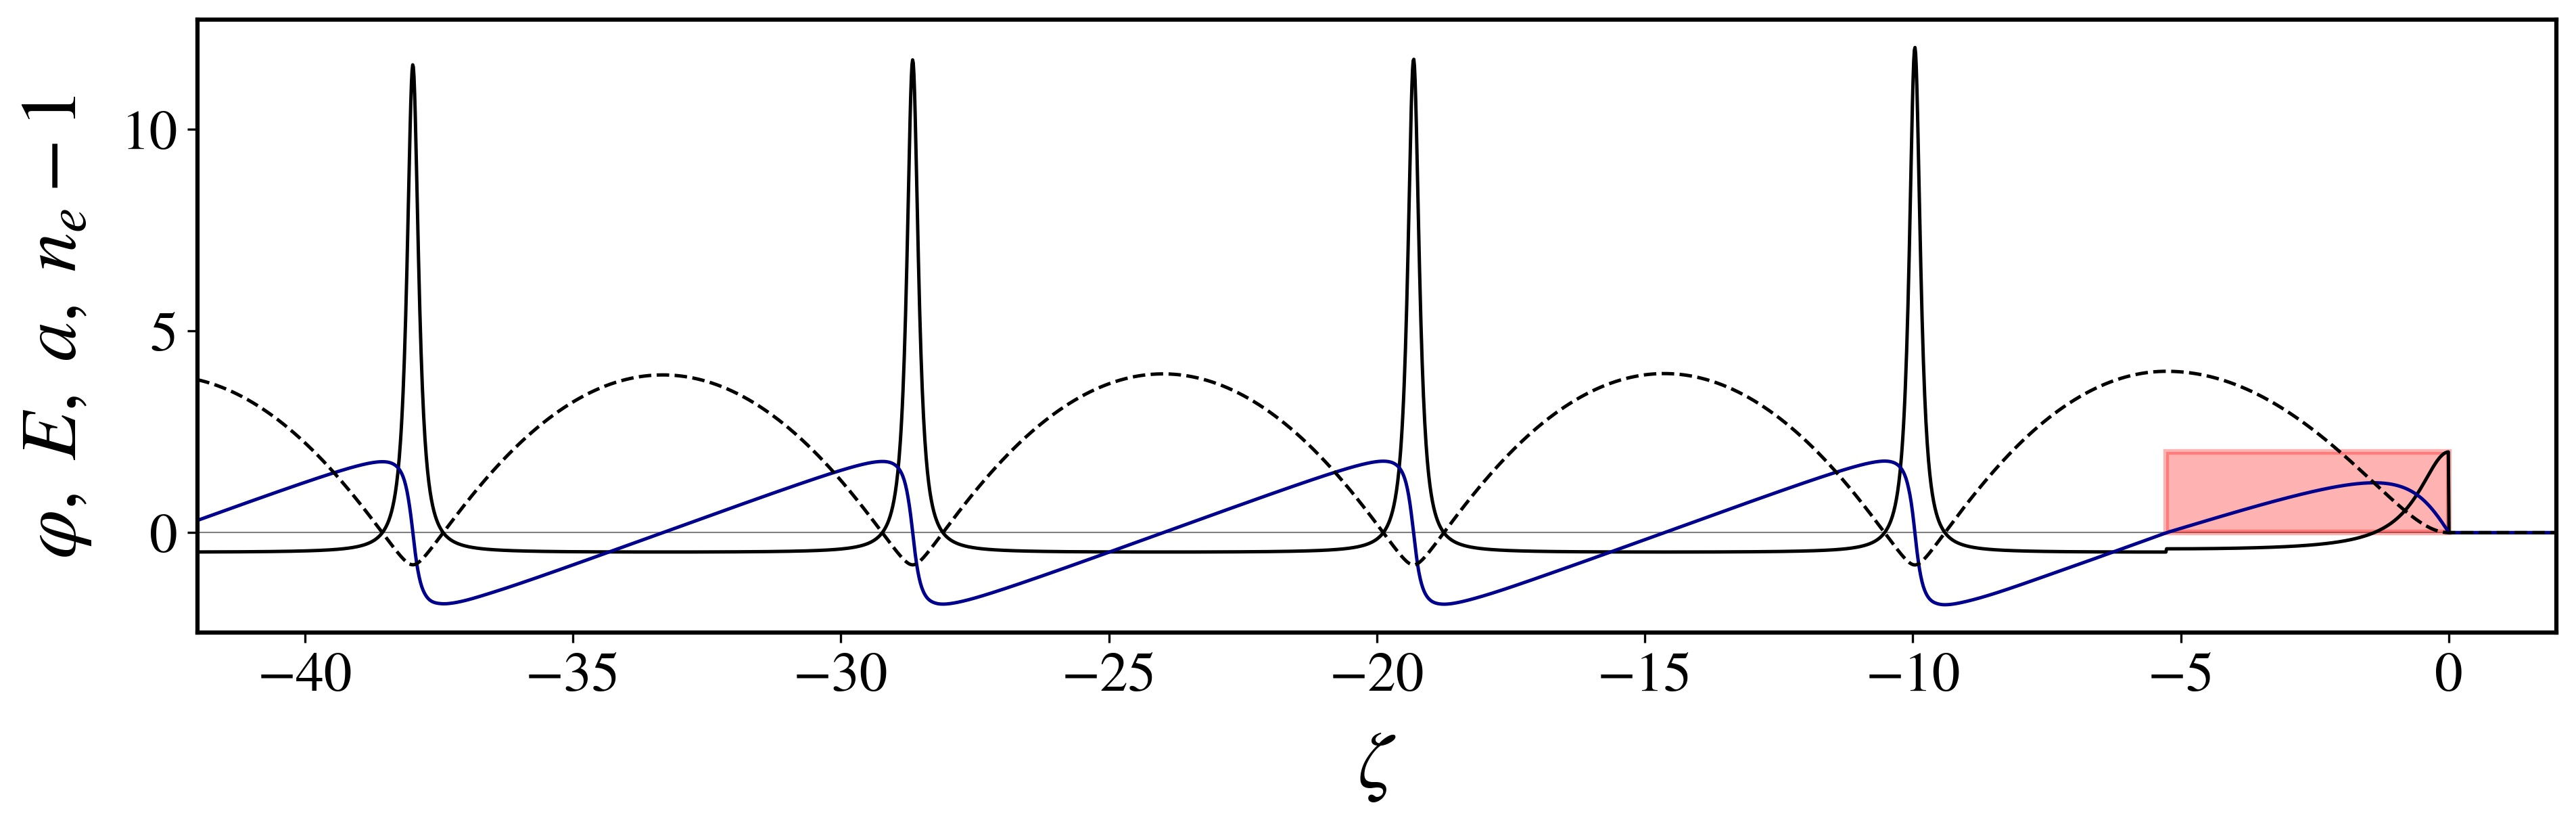
\includegraphics[width=0.9\linewidth]{img/langmuir_wave.jpg}
	\caption[]{\label{fig:} Dependence of scalar potential (black dashed line), electric field (blue), and electron density (solid black line) on the coordinate $ \zeta $ for the Langmuir wave generated by square electromagnetic pulse (red) with amplitude $ a = 2 $ and optimal length ($ l_{opt} = 5.27 $) given by Eq.~(\ref{eq:optimal_length}). The values of scalar potential and electric field in the wake left behind the driving electromagnetic pulse vary from $ -0.8 $ to $ 4 $ and from $ \approx -1.79 $ to $ \approx 1.79 $, respectively. The quantities are obtained numerically from Eq.~(\ref{eq:eq_for_scalar_potential_5}).}
\end{figure}

\subsection{Breaking of Langmuir waves}

The amplitude of the electric field in the Langmuir wave with a given value of $ \beta_w $ cannot be arbitrarily large. It has been found that if the electric field exceeds the Akhiezer-Polovin limit value of the field \cite{Akhiezer1956}, 
\begin{equation}\label{key}
E_{\mathrm{AP}} = \sqrt{2 \left( \gamma_w - 1 \right)},
\end{equation}
the Langmuir wave breaks. Here $ \gamma_w = 1 / \sqrt{1 - \beta_w^2} $ stands for the Lorentz factor of the Langmuir wave. 

In this section we discuss the properties of Langmuir waves generated by a strong electromagnetic pulse as they approach the threshold of wave breaking. Eqs.~(\ref{eq:eq_for_scalar_potential}) - (\ref{eq:eq_for_momentum}) can be rewritten in a single ordinary differential equation for the longitudinal component of the electron momentum $ p_e $ \cite{Panchenko2008, Bulanov2013},
\begin{equation}\label{eq:eq_for_long_momentum}
\diff*[2]{\left( \gamma_e - \beta_w p_e \right)}{\zeta} = \frac{p_e}{\beta_w \gamma_e - p_e},
\end{equation}
where we assume that $ \gamma_e = \sqrt{1 + p_e^2 + a^2} $ (see also Sec.~\ref{label}). One can immediately see that Eq.~(\ref{eq:eq_for_long_momentum}) becomes singular when the denominator on the right-hand side vanishes, i.e., when the electron velocity, $ p_e / \gamma_e $, approaches the phase velocity of the Langmuir wave, $ \beta_{w} $. This singularity, which is also known as the gradient or cusp catastrophe, corresponds to the breaking of Langmuir wave.

The structure of the breaking Langmuir wave can be revealed by expanding $ \gamma_e $ and $ p_e $ in the vicinity of the singularity, $ \zeta = \zeta_{br} + \delta \zeta  $, where $ \zeta_{br} $ is the breaking coordinate and $ \delta \zeta / \zeta_{br} \ll 1 $. The electron momentum is expanded as $ p_e = p_{br} + \delta p $, where $ p_{br} = \beta_w \gamma_w \sqrt{1 + a_{br}^2} $, $ \delta p / p_{br} \ll 1 $, and $ a_{br} = a \left( \zeta_{br} \right) $. From Eq.~(\ref{eq:eq_for_long_momentum}) one gets \cite{Panchenko2008, Bulanov2013}
\begin{equation}\label{eq:eq_for_long_momentum_2}
\diff*[2]{\delta p^2 }{\zeta} = -2 \beta_w \gamma_w^6 \left( 1 + a_{br}^2 \right) \delta p^{-1}.
\end{equation}
After integrating Eq.~(\ref{eq:eq_for_long_momentum_2}) over $ \zeta $ we obtain \cite{Panchenko2008, Bulanov2013}
\begin{equation}\label{eq:eq_for_long_momentum_3}
\left( \delta p \diff*{\delta p}{\zeta} \right)^2 + 2 \beta_w \gamma_w^6 \left( 1 + a_{br}^2 \right) \delta p = C,
\end{equation}
where $ C $ is the integration constant (note that the value of $ C $ can be different in regions $ \delta \zeta < 0 $ and $ \delta \zeta > 0 $ since Eq.~(\ref{eq:eq_for_long_momentum_2}) is singular at $ \delta \zeta \rightarrow 0 $).

When the product $ \delta p \, \diff{\delta p}/{\zeta} \rightarrow 0 $ at $ \delta p \rightarrow 0 $, which implies that $ C = 0 $, then \cite{Panchenko2008, Bulanov2013}
\begin{equation}\label{eq:eq_for_delta_p}
\delta p = -\beta_w \gamma_w^2 \left( \sqrt{\frac{9}{2}} \sqrt{1 + a_{br}^2} \frac{\delta \zeta}{\beta_w} \right)^{2/3}.
\end{equation}
The expression for the longitudinal electron velocity, $ \beta_e $, then reads as \cite{Panchenko2008, Bulanov2013}
\begin{equation}\label{eq:eq_for_long_velocity}
	\beta_e = \beta_w - \frac{\beta_w}{\gamma_w} \left( \sqrt{\frac{9}{2}} \left( 1 + a_{br}^2 \right)^{1/4} \frac{\delta \zeta}{\beta_w} \right)^{2/3}.
\end{equation}
Finally, by plugging Eq.~(\ref{eq:eq_for_long_velocity}) into the solution to Eq.~(\ref{eq:eq_for_density}), we obtain the distribution of the electron density, $ n_e $, as \cite{Panchenko2008, Bulanov2013}
\begin{equation}\label{eq:eq_for_density_breaking}
n_e = \frac{\beta_w}{\beta_w - \beta_e} \approx \gamma_w \left( \sqrt{\frac{2}{9}} \left( 1 + a_{br}^2 \right)^{1/4} \frac{ \beta_w}{\delta \zeta} \right)^{2/3}.
\end{equation}
Although for $ \delta \zeta \rightarrow 0 $ the electron density tends to infinity, the singularity is integrable. This means that in the breaking Langmuir wave there is a finite number of electrons \cite{Panchenko2008, Bulanov2013}.

\begin{figure}[t]
	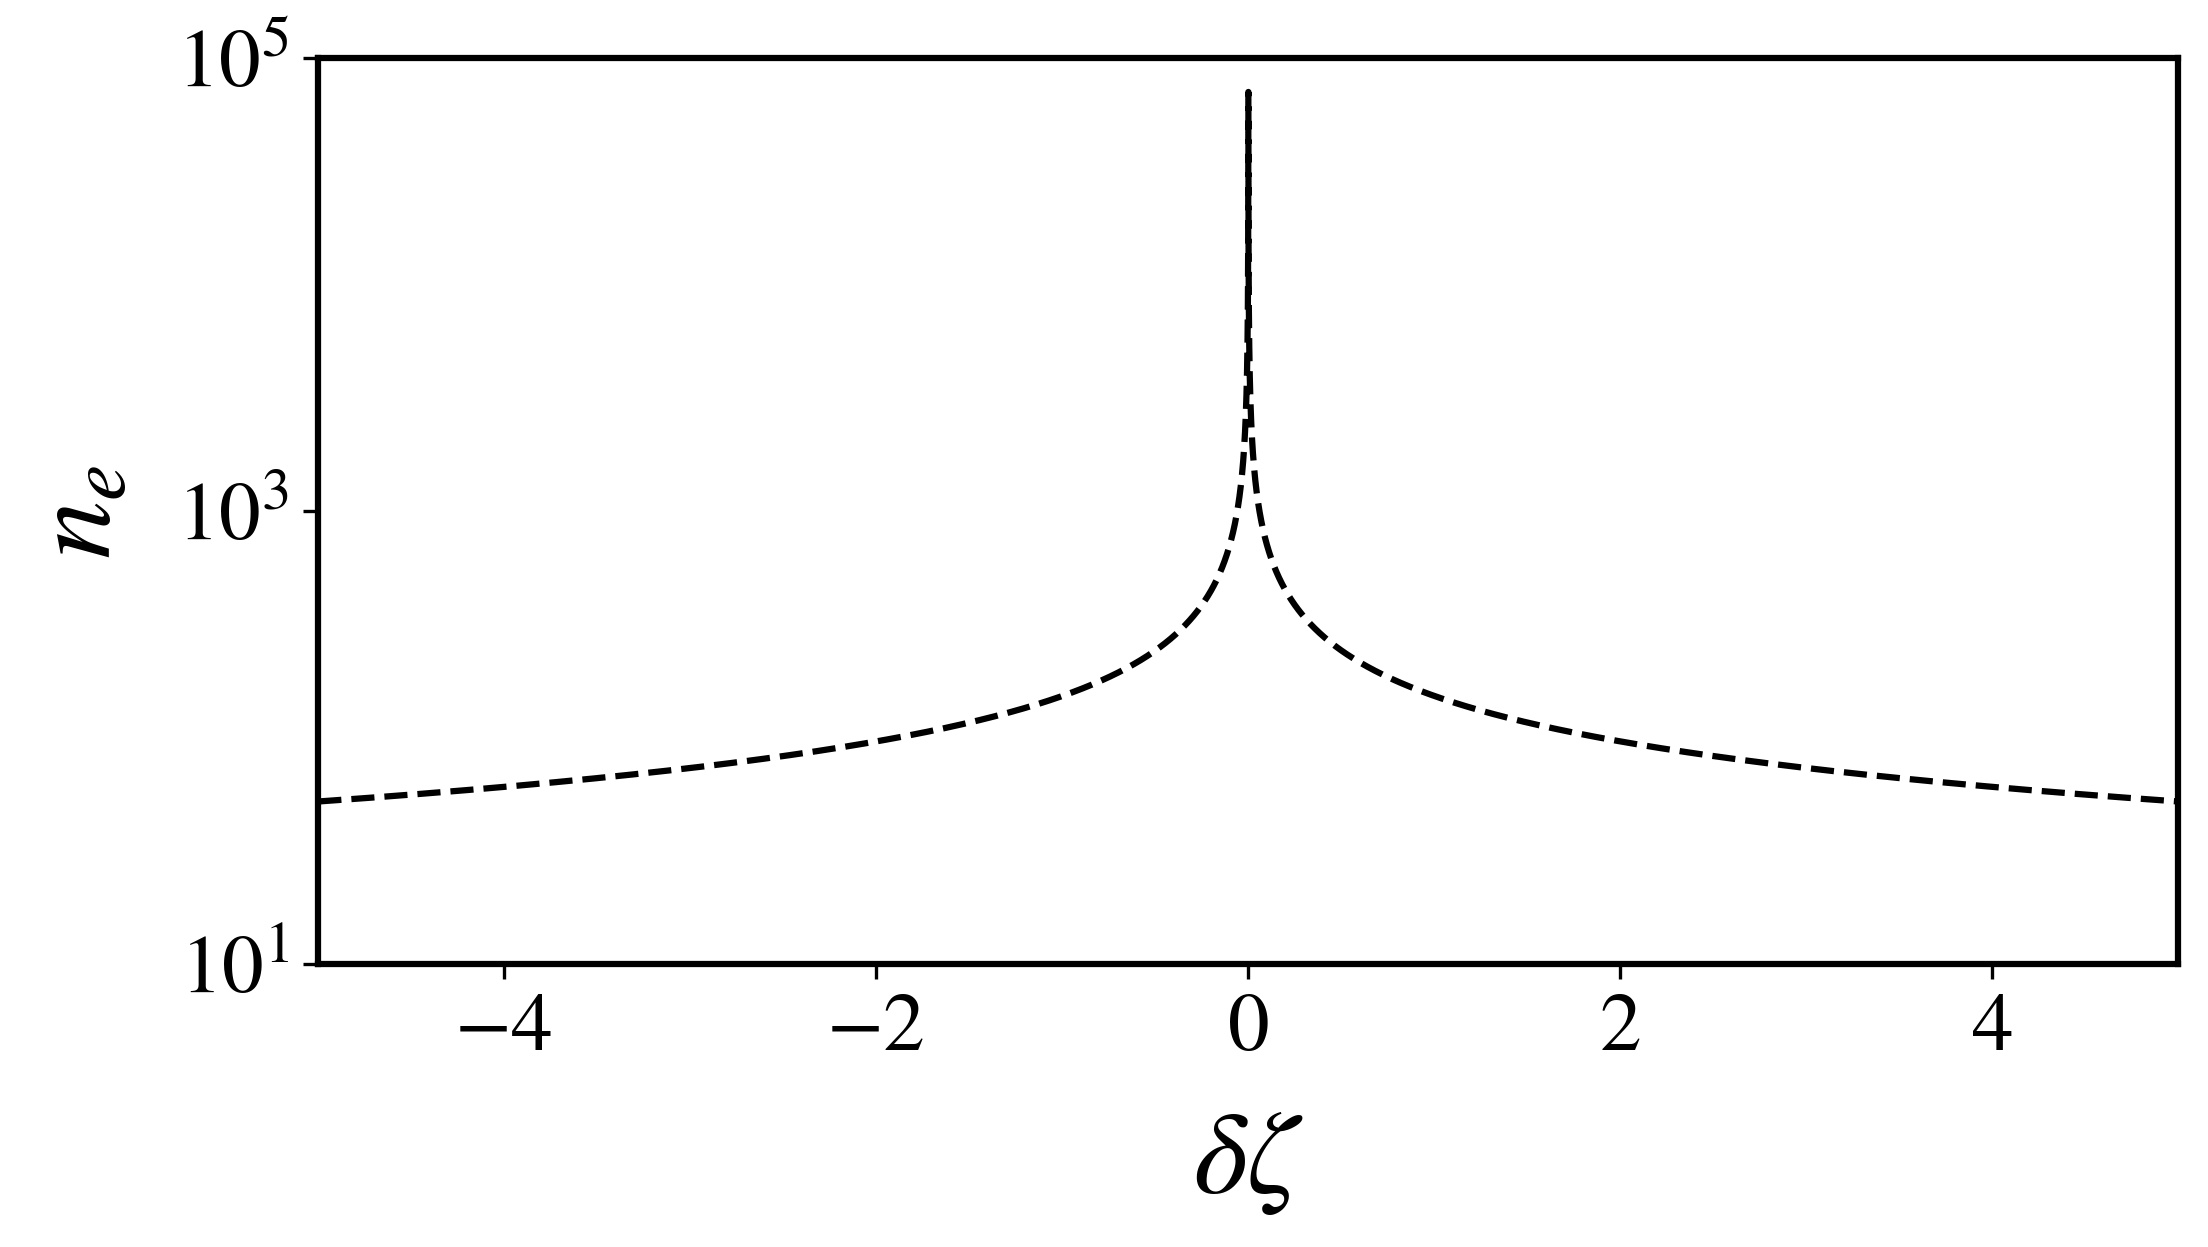
\includegraphics[width=0.5\linewidth]{img/breaking_wave.jpg}
	\caption[]{\label{fig:} Distribution of electron density of the breaking Langmuir wave near the singularity according to Eq.~(\ref{eq:eq_for_density_breaking}).}
\end{figure}

Singularities form naturally in the plasma flow with inhomogeneous velocity. There have been identified several kinds of singularities due to the breaking of finite-amplitude Langmuir waves depending on the closeness to the wave breaking threshold. It turned out that the dependence of the electron density on the coordinate can be in general expressed as $ n_e \left( \delta \zeta \right) \approx \delta \zeta^{-\alpha} $ with $ 1/2 \leq \alpha < 1 $ \cite{Panchenko2008}.


%\subsection{Self-focusing, self-guiding, self-phase modulation, self-amplitude modulation}
%\input{dat/1-0.tex}

%-------------------------------------------------------------------------------

\section{Laser-wakefield acceleration of electrons\label{sec:lwfa}}
%\input{dat/1-0.tex}

%\subsection{Electron interaction with Langmuir wave}
%\input{src/electron_interaction_with_langmuir_wave.tex}

%\subsection{Electron injection mechanisms}
%\input{dat/1-0.tex}

%\subsection{Injection by breaking plasma wave}
%\input{dat/1-0.tex}

%\subsubsection{Homogeneous plasma}
%\input{dat/1-0.tex}

%\subsubsection{Inhomogeneous plasma}
%\input{dat/1-0.tex}

%\subsection{Optical injection}
%\input{dat/1-0.tex}

%\subsection{Ionization injection}
%\input{dat/1-0.tex}

%\subsection{Regimes of LWFA}
%\input{dat/1-0.tex}

%\subsection{Self-modulated regime}

%\subsection{Blow-out regime}

%\subsection{Limitations of LWFA}
%\input{dat/1-0.tex}

%\subsection{Electron dephasing length}

%\subsection{Pump depletion length}

%\subsection{Beam loading}

%\subsection{Applications of accelerated electrons}
%\input{dat/1-0.tex}

%-------------------------------------------------------------------------------

\section{Relativistic mirrors in underdense plasmas\label{sec:rfm}}
%\input{dat/1-0.tex}

%\subsection{Lorentz transform, Doppler effect}
%\input{dat/1-0.tex}

%\subsection{Uniformly moving mirror}
%\input{dat/1-0.tex}

%\subsection{Accelerated mirror}
%\input{dat/1-0.tex}

%\subsection{Oscillating mirror}
%\input{dat/1-0.tex}

%\subsection{Physical realization of relativistic mirrors in underdense plasma}
%\input{dat/1-0.tex}

%\subsection{Langmuir wave}
%\input{dat/1-0.tex}

%\subsection{Bow wave}
%\input{dat/1-0.tex}

In this section, we describe fundamental physical processes related to the interaction of electromagnetic waves with counter-propagating relativistic mirrors. We outline a possible physical realization as well as characteristics of the mirrors in underdense plasmas which are of great interest in the context of the development of coherent high-brightness radiation sources with wavelengths ranging from x-rays to gamma-rays. For a comprehensive study about the relativistic mirrors in plasmas we refer the reader to review articles \citenum{Bulanov2013} and \citenum{Bulanov2016b}.


\subsection{Relativistic flying flat mirror\label{sec:rffm}}

%Since then, relativistic mirrors have been studied in many different contexts because of their great potential for both fundamental science and practical applications. 

First, we present a model of relativistic flying flat mirror which gives us a basic knowledge about the optical properties of reflected electromagnetic wave. The corresponding theory for the mirror propagating in vacuum at arbitrary (subluminal) velocity is known since 1905 \cite{Einstein1905}. The theory is based on the application of the Lorentz transformation formalism, where the changes in the properties of reflected electromagnetic wave are explained by the double Doppler effect.

Let us consider an ideal relativistic flying flat mirror (i.e., the mirror reflection coefficient is equal to unity, no recoil effects on reflection) moving along the $ +z $-axis at a constant velocity $ v_M = \beta_M c $. An electromagnetic wave packet linearly polarized along the $ x $-axis is counter-propagating to the mirror (i.e., moving along the $ -z $-axis). The wave packet consists of a superposition of monochromatic waves, thus its electric field can be expressed in a stationary frame of reference, $ S_1 $, using the Fourier transformation,
\begin{equation}\label{eq:incident_lab_frame_1}
\begin{split}
\vec{E}_i \left(x, y, z; t \right) &= \vec{e}_x \int_{-\infty}^{+\infty} \tilde{E}_0 \left(x, y \right) \exp \left[ -\frac{\left( \omega - \omega_0 \right)^2}{2 \Delta \omega^2} \right] \exp \left[ i \omega \left(t + \frac{z}{c}\right) \right] d \omega \\
&= \vec{e}_x \, E_0 \left(x, y \right) \exp \left[ - \frac{1}{2 \tau^2} \left(t + \frac{z}{c}\right)^2 \right] \exp \left[ i \omega_0 \left(t + \frac{z}{c}\right) \right],
\end{split}
\end{equation}
where $ \omega $, $ \omega_0 $, and $ \Delta \omega $ are, respectively, the angular frequency, center angular frequency, and the spectral bandwidth of the wave packet, $ \tilde{E}_0 \left(x, y \right) $ and $ E_0 \left(x, y \right) = \sqrt{2 \pi} \Delta \omega \tilde{E}_0 \left(x, y \right) $ are the electric field amplitudes in the spectral and time domains, respectively, and $ \tau = 1 / \Delta \omega $ is the wave packet duration (note that the full-width-at-half-maximum duration can be obtained as $ \tau_{\mathrm{FWHM}} = 2 \sqrt{2 \ln 2} \tau $).

%, where $ c $ denotes the velocity of light in vacuum
%The hat symbol refers to the unit vector.

Now we find the electric field of the incident wave packet, Eq.~(\ref{eq:incident_lab_frame_1}), in the frame of reference moving with the mirror, $ M $, through the Lorentz transformation. The Lorentz transformation of coordinates is given by
\begin{equation}\label{eq:lorentz_transform_coords}
x^{\prime} = x, \quad y^{\prime} = y, \quad z^{\prime} = \frac{z - \beta_M c t}{\sqrt{1 - \beta_M^2}}, \quad t^{\prime} = \frac{t - \frac{\beta_M}{c} z}{\sqrt{1 - \beta_M^2}}.
\end{equation}
The components of electric field transform as
\begin{equation}\label{eq:lorentz_transform_fields}
\vec{E}^{\prime}_{i, \parallel} = \vec{E}_{i, \parallel}, \quad \vec{E}^{\prime}_{i, \bot} = \frac{\vec{E}_{i, \bot} + \beta_M c \, \vec{e}_z \times \vec{B}_{i}}{\sqrt{1 - \beta_M^2}},
\end{equation}
where the subscripts $ \parallel $ and $ \bot $ denote the field polarization components parallel and perpendicular to the direction of mirror motion and $ \vec{B}_{i} = -\vec{e}_z / c \times \vec{E}_i $ is the magnetic field of the incident wave packet in $ S_1 $. Note that the origin of $ M $ is located at $ \left( 0, 0, z_0 \right) $. In $ M $, the electric field of the incident wave packet, Eq.~(\ref{eq:incident_lab_frame_1}) takes the following form,
\begin{equation}\label{eq:incident_boost_frame}
\vec{E}^{\prime}_i \left(x^{\prime}, y^{\prime}, z^{\prime}; t^{\prime} \right) = \vec{e}_x^{\prime} E^{\prime}_0 \left(x^{\prime}, y^{\prime} \right) \exp \left[ - \frac{1}{2 \tau^{\prime 2}} \left(t^{\prime} + \frac{z^{\prime}}{c}\right)^2 \right] \exp \left[ i \omega_0^{\prime} \left(t^{\prime} + \frac{z^{\prime}}{c}\right) \right],
\end{equation}
where
\begin{equation}\label{eq:coeff_boost}
E^{\prime}_0 \left(x^{\prime}, y^{\prime} \right) = \sqrt{\frac{1 + \beta_M}{1 - \beta_M}} E_0 \left(x, y \right), \quad \tau^{\prime} = \sqrt{\frac{1 - \beta_M}{1 + \beta_M}} \tau, \quad \omega_0^{\prime} = \sqrt{\frac{1 + \beta_M}{1 - \beta_M}} \omega_0.
\end{equation}

As the incident wave packet experiences reflection from the mirror, its propagation direction reverses. The electric field of the reflected wave packet in $ M $ is thus given by
\begin{equation}\label{eq:reflected_boost_frame}
\vec{E}^{\prime}_r \left(x^{\prime}, y^{\prime}, z^{\prime}; t^{\prime} \right) = \vec{e}_x^{\prime} E^{\prime}_0 \left(x^{\prime}, y^{\prime} \right) \exp \left[ - \frac{1}{2\tau^{\prime 2}} \left(t^{\prime} - \frac{z^{\prime}}{c}\right)^2 \right] \exp \left[ i \omega_0^{\prime} \left(t^{\prime} - \frac{z^{\prime}}{c}\right) \right].
\end{equation}
Now we find the electric field of the reflected wave packet, Eq.~(\ref{eq:reflected_boost_frame}), in another stationary reference frame, $ S_2 $, the origin of which coincides with the origin of $ M $, through the inverse Lorentz transformation. The inverse Lorentz transformation of coordinates is given by
\begin{equation}\label{eq:inverse_lorentz_transform_coords}
x^{\prime \prime} = x^{\prime}, \quad y^{\prime \prime} = y^{\prime}, \quad z^{\prime \prime} = \frac{z^{\prime} + \beta_M c t^{\prime}}{\sqrt{1 - \beta_M^2}}, \quad t^{\prime \prime} = \frac{t^{\prime} + \frac{\beta_M}{c} z^{\prime}}{\sqrt{1 - \beta_M^2}}.
\end{equation}
The components of electric field transform as
\begin{equation}\label{eq:inverse_lorentz_transform_fields}
\vec{E}^{\prime \prime}_{r, \parallel} = \vec{E}^{\prime}_{r, \parallel}, \quad \vec{E}^{\prime \prime}_{r, \bot} = \frac{\vec{E}^{\prime}_{r, \bot} - \beta_M c \, \vec{e}_z \times \vec{B}^{\prime}_{r}}{\sqrt{1 - \beta_M^2}},
\end{equation}
where $ \vec{B}^{\prime}_{r} = \vec{e}_z / c \times \vec{E}^{\prime}_r $ is the magnetic field of the reflected wave packet in $ M $. In $ S_2 $, the electric field of the reflected wave packet reads as
\begin{equation}\label{eq:reflected_lab_frame_1}
\vec{E}^{\prime \prime}_r \left(x^{\prime \prime}, y^{\prime \prime}, z^{\prime \prime}; t^{\prime \prime} \right) = \vec{e}_x^{\prime \prime} E^{\prime \prime}_0 \left(x^{\prime \prime}, y^{\prime \prime} \right) \exp \left[ - \frac{1}{2 \tau^{\prime \prime 2}} \left(t^{\prime \prime} - \frac{z^{\prime \prime}}{c}\right)^2 \right] \exp \left[ i \omega_0^{\prime \prime} \left(t^{\prime \prime} - \frac{z^{\prime \prime}}{c}\right) \right],
\end{equation}
where
\begin{equation}\label{eq:coeff_lab}
E^{\prime \prime}_0 \left(x^{\prime \prime}, y^{\prime \prime} \right) = \sqrt{\frac{1 + \beta_M}{1 - \beta_M}} E^{\prime}_0 \left(x^{\prime}, y^{\prime} \right), \quad \tau^{\prime \prime} = \sqrt{\frac{1 - \beta_M}{1 + \beta_M}} \tau^{\prime}, \quad \omega_0^{\prime \prime} = \sqrt{\frac{1 + \beta_M}{1 - \beta_M}} \omega_0^{\prime}.
\end{equation}

Finally, since $ x^{\prime \prime} = x $, $ y^{\prime \prime} = y $, $ z^{\prime \prime} = z - z_0 $, and $ t^{\prime \prime} = t $,
we may express the electric field of the reflected wave, Eq.~(\ref{eq:reflected_lab_frame_1}), in the original stationary reference frame, $ S_1 $, as
\begin{equation}\label{eq:reflected_lab_frame_2}
\begin{split}
\vec{E}^{\prime \prime}_r \left(x, y, z; t \right) = & \ \vec{e}_x \frac{1 + \beta_M}{1 - \beta_M} E_0 \left(x, y \right) \exp \left[ - \left(\frac{1 + \beta_M}{1 - \beta_M}\right)^2 \frac{1}{2 \tau^2} \left(t - \frac{z - z_0}{c}\right)^2 \right] \\ 
& \times \exp \left[ i \frac{1 + \beta_M}{1 - \beta_M} \omega_0 \left(t - \frac{z - z_0}{c}\right) \right].
\end{split}
\end{equation}
For a Gaussian beam of width $ w_0 $, $ E_0 \left( x, y \right) = E_0 \exp \left[-\left( x^2 + y^2 \right) / 2 w_0^2 \right] $, and thus the total energy and peak intensity of the reflected pulse is given by 
\begin{equation}\label{eq:energy_and_intensity}
\mathcal{E}^{\prime \prime}_r = \left(\frac{1 + \beta_M}{1 - \beta_M}\right) \sqrt{\frac{\pi^3}{4}} \varepsilon_0 c \tau w_0^2 E_0^2 , \quad I^{\prime \prime}_r = \left(\frac{1 + \beta_M}{1 - \beta_M}\right)^2 \frac{\varepsilon_0 c}{2} E_0^2.
\end{equation}
Note that the factor $ \left(1 + \beta_M \right) / \left(1 - \beta_M \right) $ can be rewritten in terms of the Lorentz factor of the mirror, $ \gamma_M = 1 / \sqrt{1 - \beta_M^2} $, as follows,
\begin{equation}\label{eq:factor}
\frac{1 + \beta_M}{1 - \beta_M} = \frac{\gamma_M + \sqrt{\gamma_M^2 - 1}}{\gamma_M - \sqrt{\gamma_M^2 - 1}} \approx 4 \gamma_M^2,
\end{equation}
where the last term is obtained using the identities $ \gamma_M + \sqrt{\gamma_M^2 - 1} = ( \gamma_M - \sqrt{\gamma_M^2 - 1} )^{-1} $ and $ \sqrt{\gamma_M^2 - 1} \approx \gamma_M $ and is valid in the relativistic limit, i.e., when $ \gamma_M \gg 1 $.

The above derivation shows that the reflected wave packet in the stationary frame of reference possesses several remarkable features: in the relativistic limit, its electric field is amplified by the factor $ \approx 4 \gamma_M^2 $, its duration is compressed by $ \approx 4 \gamma_M^2 $, and its angular frequency is upshifted by $ \approx 4 \gamma_M^2 $. Furthermore, its energy and intensity are enhanced by $ \approx 4 \gamma_M^2 $ and $ \approx 16 \gamma_M^4 $, respectively. Assuming a laser pulse with parameters corresponding to a typical $ \mathrm{PW} $-class titanium-doped sapphire system, i.e., $ 0.8 \ \mathrm{\mu m} $ wavelength, $ 30 \ \mathrm{fs} $ duration, and $ 10^{18} \ \mathrm{W / cm^2} $ peak intensity, being reflected from ideal relativistic flying flat mirror with $ \gamma_M = 10 $, one obtains a pulse of wavelength $ 2 \ \mathrm{nm} $, duration $ 75 \ \mathrm{as} $, and the peak intensity $ 1.6 \times 10^{23} \ \mathrm{W / cm^2} $.

\subsection{Relativistic flying parabolic mirror\label{sec:rfpm}}

%$ E_0 \left( \rho \right) $ can be thought of as the Laguerre-Gaussian function since the profiles of radially or azimuthally polarized beams can be expressed as the superposition of Laguerre-Gaussian modes (i.e., $ E_0 \sim \left(\rho / \rho_0 \right) \exp \left( - \rho^2 / 2 \rho_0^2 \right)$), 

Second, we present a model of relativistic flying parabolic mirror which, in addition to the flat mirror, describes the effect of focusing. The idea of using flying parabolic mirrors for the intensification of light has been first proposed in Ref.~\citenum{Bulanov2003}, where the mirror is realized by high-density electron shells of strongly nonlinear Langmuir wave driven by intense laser in underdense plasma (note that the surface where the electron density is maximal naturally takes a shape close to a paraboloid \cite{Bulanov1991, Bulanov1995, Matlis2006, Shadwick2002, Maksimchuk2008}).

Let us consider an ideal relativistic flying parabolic mirror (i.e., the reflection coefficient equal to unity, no recoil effects, no wavefront aberration) moving along the $ +z $-axis at a constant velocity $ v_M = \beta_M c $. The spatiotemporal distribution of the electromagnetic wave packet reflected from the mirror can be again obtained by calculating first the distribution in the moving frame of reference and then performing the transformation back to the stationary frame. It is important to note that the focal length of the parabolic mirror in the moving frame is $ \gamma_M $ times shorter than in the stationary frame \cite{Bulanov2011, Jeong2021}; this alters the situation to the $ 4 \pi $-spherical focusing scheme \cite{Gonoskov2012, Jeong2020}. The distribution of the electromagnetic fields in the focal region of parabolic mirror in the moving frame has to be thus calculated under the conditions of $ 4 \pi $-spherical focusing.

The $ 4 \pi $-spherical focusing scheme corresponds to an extreme case of either tight-focusing (where the $ f $-number approaches zero) or multiple beam focusing (where the number of beams approaches infinity). Therefore, it provides a theoretical limit to maximum attainable field strength at a given power \cite{Jeong2020}. Under the conditions of $ 4 \pi $-spherical focusing, the field distributions are obtained by calculating the vector diffraction integrals. In what follows, we assume that the electromagnetic wave packet incident on the mirror is radially or azimuthally polarized (for this case the diffraction integrals can be calculated analytically). The electric field of the incident wave packet can be thus again described by Eq.~(\ref{eq:incident_lab_frame_1}), where $ E_0 \left(x, y \right) $ can be thought of as the Laguerre-Gaussian function, i.e., $ E_0 \sim \left( \rho / \rho_0 \right)\exp \left( - \rho^2 / 2 \rho_0^2 \right)$. Here we also introduce spherical coordinates $ \rho = \sqrt{x^2 + y^2 + z^2} $ (the radial coordinate), $ \theta = \arccos \left( z / \rho \right)$ (the polar coordinate), and $ \phi = \arctan \left( y / x \right)$ (the azimuthal coordinate).

The mathematical expressions shown below cover only the case of radially polarized wave packet (the field distributions of the azimuthally polarized wave packet can be easily obtained by exchanging the expressions for the electric and magnetic fields of the radially polarized wave packet). Radial polarization is also interesting in the sense that the field distribution at focus forms a compact spot producing the maximum intensity (in contrast to, e.g., linear polarization which generates multiple intensity peaks instead).

In the moving frame of reference, the electric and magnetic fields of the $ 4 \pi $-spherical focused radially polarized wave packet are expressed in the frequency domain as \cite{Jeong2020, Jeong2021}
\begin{subequations}
\begin{equation}\label{key}
\vec{E}^{\prime}_{f} \left( \rho^{\prime}, \theta^{\prime}; \omega \right) = \vec{e}_{\theta}^{\prime} \, i E_{0, f} \left( \omega^{\prime} \right) S_a \left( \rho^{\prime}, \theta^{\prime}; \omega^{\prime} \right) \exp \left(i \omega^{\prime} t^{\prime} \right),
\end{equation}
\begin{equation}\label{key}
\vec{B}^{\prime}_{f} \left( \rho^{\prime}, \theta^{\prime}; \omega \right) = - \vec{e}_{\phi}^{\prime} \, B_{0, f} \left( \omega^{\prime} \right) S_b \left( \rho^{\prime}, \theta^{\prime}; \omega^{\prime} \right) \exp \left(i \omega^{\prime} t^{\prime} \right),
\end{equation}
\end{subequations}
where $ E_{0, f} \left( \omega^{\prime} \right) $ and $ B_{0, f} \left( \omega^{\prime} \right) $ are the peak amplitudes of the electric and magnetic fields at focus at a certain frequency $ \omega^{\prime} $, and $ S_a \left( \omega^{\prime} \right) $ and $ S_b \left( \omega^{\prime} \right) $ are the spatial distribution functions defined as \cite{Jeong2020, Jeong2021}
\begin{subequations}
	\begin{equation}\label{key}
S_a \left( \omega^{\prime} \right) = \sum_{k = 0}^{+\infty} \frac{4k + 1}{2^{3k}} j_{2k} \left( \frac{\omega^{\prime}}{c} \rho \right) P_{2k} \left( \cos \theta^{\prime} \right),
	\end{equation}
	\begin{equation}\label{key}
S_b \left( \omega^{\prime} \right) = \frac{4}{\pi} j_1 \left( \frac{\omega^{\prime}}{c} \rho \right) P^1_1 \left( \cos \theta^{\prime} \right).
	\end{equation}
\end{subequations}
Here $ j_{n} \left( \cdot \right) $ is the $ n $-th order spherical Bessel function of the first kind, and $ P_n \left( \cdot \right) $ and $ P^m_n \left( \cdot \right) $ are the Legendre and associated Legendre functions \cite{Gradshteyn1980}.

The resultant expressions for the spatiotemporal distribution of electric and magnetic fields of the radially polarized wave packet in the focal region of the mirror in the stationary frame of reference are obtained through the inverse Lorentz transformation and a Fourier transformation in the frequency domain \cite{Jeong2021},
\begin{subequations}
\begin{equation}\label{eq:reflected_e_lab_frame_parabolic}
\begin{aligned}
\vec{E}^{\prime \prime}_{f} & \left(\rho, \theta, \phi; t \right) = \gamma_M \frac{1 + \beta_M}{1 - \beta_M} \sqrt{\frac{3 \pi^5}{8}} \frac{w_e}{\lambda_0} E_0 \\[2mm]
\times &
\begin{bmatrix}
	\left\lbrace -j_0 \left( \omega_0^{\prime} R / c \right) \sin \left(\omega_0^{\prime} T \right) \Upsilon_1 + \beta_M j_1 \left( \omega_0^{\prime} R / c \right) \cos \left(\omega_0^{\prime} T \right) \Upsilon_2 \right\rbrace \cos \phi \\[1mm]
	\left\lbrace -j_0 \left( \omega_0^{\prime} R / c \right) \sin \left(\omega_0^{\prime} T \right) \Upsilon_1 + \beta_M j_1 \left( \omega_0^{\prime} R / c \right) \cos \left(\omega_0^{\prime} T \right) \Upsilon_2 \right\rbrace \sin \phi \\[1mm]
	\left( 1 / \gamma_M \right) j_0 \left( \omega_0^{\prime} R / c \right) \sin \left(\omega_0^{\prime} T \right) \Upsilon_2
\end{bmatrix},
\end{aligned}
\end{equation}
\begin{equation}\label{eq:reflected_b_lab_frame_parabolic}
\begin{aligned}
\vec{B}^{\prime \prime}_{f} & \left(\rho, \theta, \phi; t \right) = \gamma_M \frac{1 + \beta_M}{1 - \beta_M} \sqrt{\frac{3 \pi^5}{8}} \frac{w_e}{\lambda_0} \frac{E_0}{c} \\[2mm]
\times & 
\begin{bmatrix}
	\left\lbrace -j_1 \left( \omega_0^{\prime} R / c \right) \cos \left(\omega_0^{\prime} T \right) \Upsilon_2 + \beta_M j_0 \left( \omega_0^{\prime} R / c \right) \sin \left(\omega_0^{\prime} T \right) \Upsilon_1 \right\rbrace \sin \phi \\[1mm]
	\left\lbrace j_1 \left( \omega_0^{\prime} R / c \right) \cos \left(\omega_0^{\prime} T \right) \Upsilon_2 - \beta_M j_0 \left( \omega_0^{\prime} R / c \right) \sin \left(\omega_0^{\prime} T \right) \Upsilon_1 \right\rbrace \cos \phi \\[1mm]
	0
\end{bmatrix}.
\end{aligned}
\end{equation}
\end{subequations}
Here $ w_e $ is the effective radius of the wave packet ($ w_e = w_0 \sqrt{2p + m + 1}$ for the $ p $-th radial, $ m $-th azimuthal Laguerre-Gaussian beam), $ \lambda_0 = 2 \pi c / \omega_0 $ is the wave packet wavelength,
\begin{subequations}
\begin{equation}\label{eq:envelope_function_1}
\begin{aligned}
\Upsilon_1 \left(T, R \right) & = \frac{1}{2} \left\lbrace \frac{\cos \theta + \beta_M}{1 + \beta_M \cos \theta} \exp \left[- \frac{\Delta \omega^{\prime 2}}{4} \left( T + \frac{R}{c} \right)^2 \right] \right. \\
+ & \left. \frac{\cos \theta - \beta_M}{1 - \beta_M \cos \theta} \exp \left[- \frac{\Delta \omega^{\prime 2}}{4} \left( T - \frac{R}{c} \right)^2 \right] \right\rbrace,
\end{aligned}
\end{equation}
\begin{equation}\label{eq:envelope_function_2}
\begin{aligned}
\Upsilon_2 \left(T, R \right) & = \frac{1}{2} \left\lbrace \frac{\sin \theta}{\gamma_M \left( 1 - \beta_M \cos \theta \right) } \exp \left[- \frac{\Delta \omega^{\prime 2}}{4} \left( T - \frac{R}{c} \right)^2 \right] \right. \\
+ & \left. \frac{\sin \theta}{\gamma_M \left( 1 + \beta_M \cos \theta \right) } \exp \left[- \frac{\Delta \omega^{\prime 2}}{4} \left( T + \frac{R}{c} \right)^2 \right] \right\rbrace
\end{aligned}
\end{equation}
\end{subequations}
are the envelope functions, and
\begin{equation}\label{eq:T_and_R}
T \left(t, \rho \right) = \frac{t - \left(\rho / c\right) \beta_M \cos \theta}{\gamma_M \left( 1 - \beta_M^2 \cos^2 \theta \right)}, \quad R \left(\rho, t \right) = \frac{\rho - c t \beta_M \cos \theta}{\gamma_M \left( 1 - \beta_M^2 \cos^2 \theta \right)}.
\end{equation}

The phase of the outgoing wave packet in the stationary frame of reference can be obtained by decomposing the spherical Bessel function in Eqs.~(\ref{eq:reflected_e_lab_frame_parabolic}) or (\ref{eq:reflected_b_lab_frame_parabolic}) as $ \omega_0^{\prime} \left( T - R / c \right) = \left[ \left( 1 + \beta_M \right) / \left( 1 - \beta_M \cos \theta \right) \right] \omega_0 \left( t - \rho / c \right) $, thus the angular frequency is given by
\begin{equation}\label{key}
	\omega_0^{\prime \prime} = \frac{1 + \beta_M}{1 - \beta_M \cos \theta} \omega_0.
\end{equation}
In the relativistic limit ($ \gamma_M \gg 1 $) and in the forward direction ($ \theta = 0 $), the angular frequency is upshifted by the factor $ \approx 4 \gamma_M^2 $, which is consistent to the case of relativistic flying flat mirror.

The spectral bandwidth of the outgoing wave packet in the stationary frame of reference is determined by the term $ \Delta \omega^{\prime 2} \left( T - R / c \right)^2 / 4 = \left[ \left( 1 + \beta_M \right) / \left( 1 - \beta_M \cos \theta \right) \right]^2 \Delta \omega^2 \left( t - \rho / c \right)^2 / 4 $ in Eqs.~(\ref{eq:envelope_function_1}) or (\ref{eq:envelope_function_2}), thus the duration is given by
\begin{equation}\label{key}
	\tau^{\prime \prime} = \frac{1 - \beta_M \cos \theta}{1 + \beta_M} \tau.
\end{equation}
Again, in the relativistic limit and the forward direction, the duration is compressed by the factor $ \approx 4 \gamma_M^2 $, consistently to the case of relativistic flying flat mirror.

From Eqs.~(\ref{eq:reflected_e_lab_frame_parabolic}) and (\ref{eq:reflected_b_lab_frame_parabolic}) it is also clear that the field strength and intensity of the reflected wave packet at focus of the relativistic flying parabolic mirror are in the relativistic limit enhanced by factors of $ \approx 4 \gamma_M^3 \sqrt{3 \pi^5 / 8} \left( w_e / \lambda_0 \right) $ and $ \approx 16 \gamma_M^6 \left( 3 \pi^5 / 8 \right) \left( w_e / \lambda_0 \right)^2 $, respectively; thus in comparison with the relativistic flying flat mirror, the focusing provides additional enhancements of the field strength and intensity of $ \approx \gamma_M \sqrt{3 \pi^5 / 8} \left( w_e / \lambda_0 \right) $ and $ \approx \gamma_M^2 \left( 3 \pi^5 / 8 \right) \left( w_e / \lambda_0 \right)^2 $, respectively. Assuming again a laser pulse of wavelength $ 0.8 \ \mathrm{\mu m} $, effective radius $ 3 \ \mathrm{\mu m} $, and peak intensity $ 10^{18} \ \mathrm{W / cm^2} $ being reflected from an ideal relativistic flying parabolic mirror with $ \gamma_M = 10 $, one obtains an intensity of $ 2.6 \times 10^{28} \ \mathrm{W / cm^2} $ at focus.

\subsection{Reflection coefficient}

%As mentioned in Sec.~\ref{sec:rfpm}, the relativistic flying mirror can be physically realized in underdense plasma by a strongly nonlinear Langmuir wave. 

In reality the reflection coefficient of relativistic flying mirrors in plasmas is, in general, very far from unity and, therefore, constitutes an important factor that has to be taken into account. Here we present an estimation of the reflection coefficient for the mirror being physically realized with strongly nonlinear Langmuir wave in underdense plasma.

Let us consider a Langmuir wave near the threshold of breaking, which moves along the $ +z $-axis at a constant phase velocity $ v_{M} = \beta_M c $. The counter-propagating electromagnetic wave incident on the mirror is characterized by the $ x $-component of the vector potential $ A_x \left( y, z; t \right) $; the interaction between the electromagnetic wave and the mirror is governed by the wave equation
\begin{equation}\label{eq:refl_coeff_vector_potential}
	\diffp[2]{A_x}{t} - c^2 \left( \diffp[2]{A_x}{y} + \diffp[2]{A_x}{z} \right) + \omega_{pe}^2 A_x = 0,
\end{equation}
where $ \omega_{pe} \left( \zeta \right) = \sqrt{e^2 n\left( \zeta \right) / \left( \varepsilon_0 m_e \gamma_e \right)} $ is the relativistic Langmuir frequency, $ \gamma_e $ is the electron Lorentz factor (note that $ \gamma_e = \gamma_M $ at the wave breaking coordinate $ \zeta_{br} $), $ n \left( \zeta \right) $ is the distribution of the electron density within the Langmuir wave, and $ \zeta = z - \beta_M c t $. 

%We assume the Langmuir wave at the wave-breaking threshold; the electron density can be thus generally described by
%\begin{equation}\label{key}
%n = \frac{n_0 G_{\alpha}}{\left( k_p \zeta \right)^{\alpha}},
%\end{equation}
%where $ n_0 $ is the ambient plasma density, $ k_p $ is the plasma wavenumber, $ G_{\alpha} $ is a dimensionless constant, and $ 1/2 \leq \alpha < 1 $. 

The form of Eq.~(\ref{eq:refl_coeff_vector_potential}) in the frame of reference moving with the mirror can be found using the Lorentz transformation as
\begin{equation}\label{eq:refl_coeff_vector_potential_2}
\frac{d^2 a}{d z^{\prime 2}}+ \left( s^2 - \nu \right) a = 0.
\end{equation}
Here $ a \left( z^{\prime} \right) $ is the vector potential normalized by $ m_e c / e $, $ s = \sqrt{ \left( \omega_0^{\prime} / c \right)^2 - k_y^{\prime 2}} $, and $ \nu \left( z^{\prime} \right) = \omega_{pe}^2\left( z^{\prime} \right) / c^2 $. We look for the solution of Eq.~(\ref{eq:refl_coeff_vector_potential_2}) in the form of
%where $ k_y^{\prime} $ is the $ y $-component of the wave vector of the incident electromagnetic wave in the moving reference frame,
\begin{equation}\label{eq:vector_potential_form}
a = b_{-} \left( z^{\prime} \right) \exp \left( -i s z^{\prime} \right) + b_{+} \left( z^{\prime} \right) \exp \left( i s z^{\prime} \right),
\end{equation}
and impose the following boundary conditions on the functions $ b_{-} \left( z^{\prime} \right) $ and $ b_{+} \left( z^{\prime} \right) $: In the limit $ z^{\prime} \rightarrow +\infty $, functions $ b_{-} \left( z^{\prime} \right) $ and $ b_{+} \left( z^{\prime} \right) $ represent the amplitudes of the incident and reflected electromagnetic waves, respectively, i.e, we set $ b_{-} \left( +\infty \right) = 1 $ and $ b_{+} \left( +\infty \right) = \rho $. In the opposite limit $ z^{\prime} \rightarrow -\infty $, $ b_{-} \left( z^{\prime} \right) $ is the amplitudes of the transmitted wave and $ b_{+} \left( z^{\prime} \right) $ vanishes, i.e, we set $ b_{-} \left( -\infty \right) = \tau $ and $ b_{+} \left( -\infty \right) = 0 $. We also require the following condition on the derivative of $ a $ to be satisfied,
\begin{equation}\label{eq:boundary_condition_1}
\diff{a}{z^{\prime}} = -i s b_{-} \exp \left( -i s z^{\prime} \right) + i s b_{+} \exp \left( i s z^{\prime} \right),
\end{equation}
which implies that
\begin{equation}\label{eq:boundary_condition_2}
\diff{b_{+}}{z^{\prime}} \exp \left( i s z^{\prime} \right) = -\diff{b_{-}}{z^{\prime}} \exp \left( -i s z^{\prime} \right).
\end{equation}

By plugging Eq.~(\ref{eq:vector_potential_form}) into Eq.~(\ref{eq:refl_coeff_vector_potential_2}) and taking into account the condition of Eq.~(\ref{eq:boundary_condition_2}), we may write a system of equations for the functions $ b_{-} $ and $  b_{+} $ in the following compact form,
\begin{equation}\label{eq:refl_coeff_system}
\diff*
{\begin{bmatrix}
	b_{-} \\
	b_{+} 
\end{bmatrix}}
{z^{\prime}} = \frac{i \nu}{2 s} 
\begin{bmatrix}
	\exp \left( 2 i s z^{\prime} \right) & 1 \\
	-1 & -\exp \left( -2 i s z^{\prime} \right)
\end{bmatrix}
{\begin{bmatrix}
	b_{-} \\
	b_{+}
\end{bmatrix}}.
\end{equation}
Assuming that the amplitude of the reflected wave is much smaller than the amplitude of the incident wave (i.e., $ \rho \ll 1 $), the solution of the system of Eqs.~(\ref{eq:refl_coeff_system}) can be written as
\begin{equation}\label{eq:eq_for_rho}
	\rho = \frac{i}{2 s} \int_{-\infty}^{+\infty} \nu \left( z^{\prime} \right) \exp \left( -2 i s z^{\prime} \right) \dl z^{\prime}.
\end{equation}

Since we consider a Langmuir wave at the threshold of wave breaking, we may use Eq.~(\ref{eq:eq_for_density_breaking}) to describe the distribution of the electron density. In the moving frame of reference, in which the Langmuir wave is at rest, this yields
\begin{equation}\label{eq:eq_for_nu}
\nu = \frac{\left( 2 / 9 \right)^{1/3} \left( 1 + a_{br}^2 \right)^{1/6} k_p^{4/3} \gamma_M^{2/3}}{\left( z^{\prime} \right)^{2/3}}.
\end{equation} 
After substituting Eq.~(\ref{eq:eq_for_nu}) into Eq.~(\ref{eq:eq_for_rho}) and calculating the integral we obtain
\begin{equation}\label{eq:eq_for_rho_2}
\rho = \frac{i 3^{1 / 2} \Gamma \left( 1 / 3 \right) \left( 2 / 9 \right)^{1/3} \left( 1 + a_{br}^2 \right)^{1/6} k_p^{4/3} \gamma_M^{2/3}}{\left( 2 s \right)^{4 / 3}},
\end{equation}
where $ \Gamma \left( \cdot \right) $ is the Euler gamma function \cite{Gradshteyn1980}. Finally, the reflection coefficient can be obtained as follows,
\begin{equation}\label{eq:reflection_coefficient}
\mathcal{R} = \norm{\rho}^2 = \frac{\Gamma^2 \left( 1 / 3 \right) \left( 1 + a_{br}^2 \right)^{1 / 3} k_p^{8/3} \gamma_M^{4/3}}{2^2 3^{1 / 3} s^{8 / 3}}.
\end{equation}
It is important to note that the formula for the reflection coefficient given by Eq.~(\ref{eq:reflection_coefficient}) is calculated in the moving frame of reference. In the stationary frame, it has to be interpreted as a reflection coefficient in terms of the photon number. 

\subsection{Recoil efects}

Furthermore, the calculations presented above are valid only if the amplitude of the electromagnetic wave incident on the relativistic mirror is sufficiently low. When the amplitude is high, the electromagnetic wave may significantly affect the mirror motion (i.e., the radiation pressure of the wave may slow down or destroy the mirror) even if the mirror reflection coefficient is small. The knowledge of the onset of recoil effects associated with the interaction of the relativistic mirror and strong incident electromagnetic wave is thus crucial for maximizing the amplitude of the reflected wave.

The recoil effects of relativistic mirrors physically realized by the structures in laser plasmas have been recently investigated in one-dimensional [\ref{paper_3}] and two-dimensional \cite{Jeong2021} geometries. Here we present the one-dimensional description. Let us consider a relativistic mirror in the form of an electron layer interacting with a counter-propagating electromagnetic wave. We assume that all the electrons are characterized by the same momentum, the electromagnetic wave is monochromatic with the angular frequency $ \omega_0 $, and the reflection coefficient (in terms of photon number) is equal to $ \mathcal{R} $. The conservation of momentum and energy before (unprimed quantities) and after (double-primed quantities) the interaction can be written as [\ref{paper_3}]
\begin{subequations}\label{eq:conservation}
\begin{equation}\label{eq:conservation_of_momentum}
\mathcal{N}_e p_e - \mathcal{N}_{\omega} p_{\omega} = \mathcal{N}_e p_e^{\prime \prime} + \mathcal{R} \mathcal{N}_{\omega} p_{\omega}^{\prime \prime} - \left( 1 - \mathcal{R} \right) \mathcal{N}_{\omega} p_{\omega},
\end{equation}
\begin{equation}\label{eq:conservation_of_energy}
\mathcal{N}_e \mathcal{E}_e + \mathcal{N}_{\omega} \mathcal{E}_{\omega} = \mathcal{N}_e \mathcal{E}_e^{\prime \prime} + \mathcal{R} \mathcal{N}_{\omega} \mathcal{E}_{\omega}^{\prime \prime} + \left( 1 - \mathcal{R} \right) \mathcal{N}_{\omega}  \mathcal{E}_{\omega}.
\end{equation}
\end{subequations}
Here $ \mathcal{N} $, $ p $, and $ \mathcal{E} $ are the numbers, momenta, and energies of the interacting particles, respectively, and the subscripts $ e $ and $ \omega $ denote the electrons (representing the relativistic flying mirror) and photons (representing the incident electromagnetic wave), respectively. The electron and photon momenta can be expressed as $ p_e = m_e c \sqrt{\gamma_M^2 - 1} $ and $ p_{\omega} = \hbar \omega_0 / c $, respectively, and the electron and photon energies are $ \mathcal{E}_e = m_e c^2 \gamma_M $ and $ \mathcal{E}_{\omega} = \hbar \omega_0 $, respectively, where $ \hbar $ stands for the reduced Planck constant. 

%The schematic of the analytical model is displayed in Fig.~\ref{fig:recoil_schematic}.

% energies can be expressed as
%\begin{subequations}\label{eq:electron_and_photon_momentum_and_energy}
%\begin{equation}\label{eq:electron_and_photon_momentum}
%p_e = m_e c \sqrt{\gamma_M^2 - 1}, \quad p_{\omega} = \hbar \omega_0 / c,
%\end{equation}
%\begin{equation}\label{eq:electron_and_photon_energy}
%\mathcal{E}_e = m_e c^2 \gamma_M, \quad \mathcal{E}_{\omega} = \hbar \omega_0,
%\end{equation}
%\end{subequations}
%where $ \hbar $ is the reduced Planck constant.

%\begin{figure}[t]
%	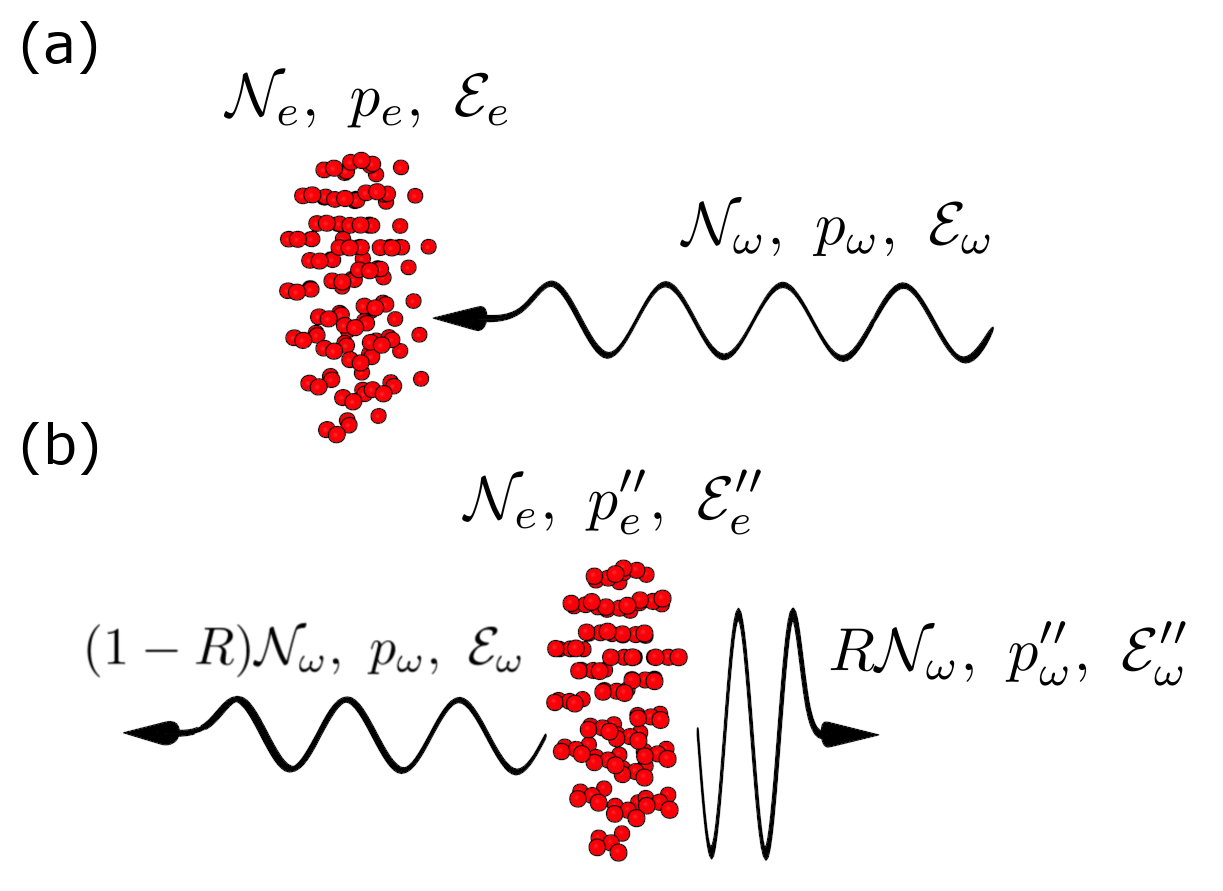
\includegraphics[width=0.45\linewidth]{img/recoil_scheme.png}
%	\caption[]{\label{fig:recoil_schematic} Schematic illustrating the analytical model of Eqs.~(\ref{eq:conservation}) (a) before and (b) after the interaction of incident electromagnetic wave with a counter-propagating relativistic mirror, which is represented by thin electron layer (red dots).}
%\end{figure}

By combining Eqs.~(\ref{eq:conservation}) we obtain the following formula [\ref{paper_3}],
\begin{equation}\label{eq:recoil_1}
\hbar \omega_0^{\prime \prime} = \hbar \omega_0 \frac{\mathcal{E}_e \left( \mathcal{E}_e + p_e c \right)}{\mathcal{N}_e \left( \mathcal{E}_e + p_e c \right) + 2 \mathcal{R} \mathcal{N}_{\omega} \hbar \omega_0} = \hbar \omega_0 \frac{\mathcal{N}_e m_e c^2 \left( \gamma_M + \sqrt{\gamma_M^2 - 1} \right)}{\mathcal{N}_e m_e c^2 \left( \gamma_M - \sqrt{\gamma_M^2 - 1} \right) + 2 \mathcal{R} \mathcal{N}_{\omega} \hbar \omega_0}.
\end{equation}
In the relativistic limit, Eq.~(\ref{eq:recoil_1}) can be simplified as
\begin{equation}\label{eq:recoil_2}
\omega_0^{\prime \prime} \approx 4 \gamma_M^2 \omega_0 \frac{\mathcal{N}_e m_e c^2 / 4 \gamma_M}{\mathcal{N}_e m_e c^2 / 4 \gamma_M + \mathcal{R} \mathcal{N}_{\omega} \hbar \omega_0} \approx 4 \gamma_M^2 \omega_0 \left( 1 - \frac{\mathcal{R} \mathcal{N}_{\omega} \hbar \omega_0}{\mathcal{N}_e m_e c^2 / 4 \gamma_M} \right).
\end{equation}
The fraction in parentheses on the right-hand side of Eq.~(\ref{eq:recoil_2}) is the ratio between the energy of interacting photons (numerator) and the energy of electron layer (denominator), and it represents the correction to the frequency shift of the reflected wave by the recoil effects. The resulting frequency shift is determined by the relationship between both terms [\ref{paper_3}],
\begin{subequations}
\begin{equation}\label{eq:recoil_limit_1}
\frac{\omega_0^{\prime \prime}}{\omega_0} \approx 4 \gamma_M^2 \quad \mathrm{if} \quad \mathcal{R} \mathcal{N}_{\omega} \hbar \omega_0 \ll \frac{\mathcal{N}_e m_e c^2}{4 \gamma_M},
\end{equation}
\begin{equation}\label{eq:recoil_limit_2}
\frac{\omega_0^{\prime \prime}}{\omega_0} \approx \frac{\mathcal{N}_e m_e c^2 \gamma_M}{\mathcal{R} \mathcal{N}_{\omega} \hbar  \omega_0} \quad \mathrm{if} \quad \mathcal{R} \mathcal{N}_{\omega} \hbar \omega_0 \gg \frac{\mathcal{N}_e m_e c^2}{4 \gamma_M}. 
\end{equation}
\end{subequations}

The limit given by Eq.~(\ref{eq:recoil_limit_1}) corresponds to the approximation of a weak incident electromagnetic wave and produces the classical frequency upshift factor as derived in Secs.~\ref{sec:rffm} and \ref{sec:rfpm}. In the opposite limit given by Eq.~(\ref{eq:recoil_limit_2}), the incident electromagnetic wave significantly affects the motion of the mirror so that the frequency of the reflected wave is in fact downshifted, as in the case of receding mirror. We define the threshold characterizing the importance of recoil effects in this interaction as a midpoint between the limits given by Eqs.~(\ref{eq:recoil_limit_1}) and (\ref{eq:recoil_limit_2}), i.e., when the energy of the interacting photons is comparable to that of the electron layer [\ref{paper_3}],
\begin{equation}\label{eq:recoil_threshold}
	\mathcal{R} \mathcal{N}_{\omega} \hbar  \omega_0 = \varkappa \frac{\mathcal{N}_e m_e c^2}{4 \gamma_M}.
\end{equation}
Here $ \varkappa \ll 1 $, i.e., much less energy than the kinetic energy of the mirror can affect the reflection process. The value of $ \varkappa $ was estimated using particle-in-cell simulations to $ \approx 10^{-4} $ for the case of relativistic mirror realized with strongly nonlinear Langmuir wave [\ref{paper_3}].



%-------------------------------------------------------------------------------

\section{Particle-in-cell algorithm}
%\input{dat/1-0.tex}

%Laser-plasma interaction involves a collective behavior of particles and electromagnetic fields which is in general complex and strongly non-linear problem to solve. The investigation of such systems cannot be usually carried out only through the theoretical and experimental work. Since a large amount of simultaneous processes with many degrees of freedom may be present there, analytical modeling seems to be impractical. On the other hand, many of the significant details of laser-plasma interaction may be extremely difficult or even impossible to obtain experimentally. Hence, other tools and techniques are required for the further progress in this field of research \cite{jaroszynsky}.

%Numerical simulations help researchers to develop models covering a wide range of physical scenarios as well as to investigate their properties. With the advent of powerful computational systems, numerical simulations now play an important role as an essential tool in developing theoretical models and understanding experimental results in various fields of modern science \cite{pang}. These so-called computer experiments are often faster and much cheaper than a single real experiment in laboratory \cite{gould}. In addition, one numerical code can solve a broad range of tasks only by modification of its initial and boundary conditions.

%Nowadays, it is clear that detailed understanding of the physical mechanisms in the laser-plasma interaction can be achieved only through the combination of theory, experiment and simulation. Development of parallel algorithms that are able to provide sufficiently exact solutions in reasonable time, however, belongs to the most challenging fields of modern science.

%Individual steps are closer described in several following sections. An extensive study of PIC method can be found in \cite{birdsall, hockney}.

\subsection{General description}

In the particle-in-cell method, the evolution of a system is determined by the motion of individual particles. However, real systems are in general very large in terms of a number of particles they contain. The particle-in-cell method therefore uses a finite set of so-called quasi-particles, each representing a group of physical particles that are near each other in the phase space. A quasi-particle becomes a carrier of certain attributes, e.g., mass, charge, position in space, momentum, etc. As shown below, it is possible to rescale the number of particles in the system, since the Lorentz force acting on the particles depends only on the charge to mass ratio, which is invariant to this transformation. 

The particle-in-cell algorithm combines the Eulerian and Lagrangian approaches of the mathematical description. The electromagnetic fields are calculated on a fixed mesh (Eulerian frame), whereas the quasi-particles can move in a continuous phase space (Lagrangian frame). The algorithm is outlined below for three-dimensional Cartesian grid, therefore we may discretize the spatial coordinate as $ \vec{r} \rightarrow \vec{r}_{i j k} $, where $ (i, \ j, \ k) \in \mathbb{Z}^{3} $ are the grid indices. If $ \Delta x $, $ \Delta y $, and $ \Delta z $ are the spatial steps in each direction, then $ \vec{r}_{i j k} = \left( i \Delta x, \ j \Delta y, \ k \Delta z \right) $. The time is discretized as $ t \rightarrow t^{\,n} $, where $ n \in \mathbb{N} $ is the time level index. If $ \Delta t $ is the time step, then $ t^{\,n} = n \Delta t $. Each quantity $ A \left(\vec{r}_{i j k}, t^{\,n} \right) $ is hereafter denoted as $ A_{ijk}^{\,n} $.

%In the case of three-dimensional geometry, the spatial coordinate is discretized as $ \vec{r} \rightarrow \vec{r}_{i j k} $, where $ (i, \ j, \ k) \in \mathbb{Z}^{3} $ are the grid indices. The time is discretized as $ t \rightarrow t^{\,n} $, where $ n \in \mathbb{N} $ is the time level index. The algorithm is outlined below for regular Cartesian grid, therefore $ \vec{r}_{i j k} = \left( i \Delta x, \ j \Delta y, \ k \Delta z \right) $, where $ \Delta x $, $ \Delta y $, and $ \Delta z $ are the spatial steps in each direction, and $ t^{\,n} = n \Delta t $, where $ \Delta t $ is the time step. Each quantity $ A \left(\vec{r}_{i j k}, t^{\,n} \right) $ is hereafter denoted as $ A_{ijk}^{\,n} $.

In kinetic theory, each particle species $ s $ in the system is assigned a distribution function $ f_{s} \left( \vec{r}, \vec{p}, t \right) $, where $ \vec{r} $ and $ \vec{p} $ denote, respectively, the position and momentum of a phase-space element, and $ t $ is time. In the case of collisionless plasma, the evolution of $ f_{s} $ is governed by the Vlasov equation
\begin{equation}\label{eq:vlasov_eq}
	\left( \diffp[]{}{t} + \frac{\vec{p}}{m_s \gamma} \cdot \nabla + \vec{F}_L \cdot \frac{\partial}{\partial \vec{p}} \right) f_s = 0,
\end{equation}
where $ \vec{F}_L = q_s \left( \vec{E} + \vec{v} \times \vec{B} \right) $ is the Lorentz force that stems from the existence of collective electric, $ \vec{E} \left( \vec{r}, t \right) $, and magnetic, $ \vec{B} \left( \vec{r}, t \right) $, fields in plasma, $ \vec{v} = \vec{p} / \left( m_s \gamma \right) $, and $ \gamma = \sqrt{1 + \vec{p}^2 / \left( m_s^2 c^2 \right)} $.

The particle-in-cell algorithm assumes that $ f_{s} $ is obtained by summing the distribution functions of each quasi-particle $ p $ of species $ s $ $ f_{p, s} \left( \vec{r}, \vec{p}, t \right) $,
\begin{equation}\label{eq:dist_function}
	f_{s} =  \sum_{p} f_{p, s}.
\end{equation}
Here and below we use the subscript $ p $ to denote the quantities attributed to quasi-particles or evaluated at the quasi-particle positions. The quasi-particle distribution function can be defined as 
\begin{equation}\label{eq:quasi_particle_dist_function}
	f_{p, s} \left( \vec{r}, \vec{p}, t \right) = w_{p} S^r \left[ \vec{r} - \vec{r}_{p} \left( t \right) \right] S^p \left[ \vec{p} - \vec{p}_{p} \left( t \right) \right],
\end{equation}
where $ S^r $ and $ S^p $ are the shape functions for the position and momentum variables, respectively, and $ w_{p} $ is the weight of the quasi-particle (i.e., a number of physical particles which the quasi-particle represents).

The shape functions cannot be chosen arbitrarily, they have to satisfy the following requirements: (i) the shape function is symmetric, (ii) the integral of the shape function is equal to unity, and (iii) the support of the shape function is compact. A standard implementation of the particle-in-cell algorithm is based on the choice of $ S^r $ as the $ m $-th order B-spline function $ b_{m} $ and $ S^p $ as the Dirac $ \delta $-function. Note that smoother shape functions are used to reduce numerical noise and non-physical fluctuations in the simulations (at the cost of increased computational time).

The equations of motion for quasi-particle $ p $ can be obtained by substituting Eq.~(\ref{eq:dist_function}) into Eq.(\ref{eq:vlasov_eq}) and taking into account the properties of shape functions mentioned above,
%\begin{equation}\label{eq:quasi_particle_eq_of_motion}
%	\diff{\vec{r}_{p}}{t} = \vec{v}_{p}, \qquad \diff{\vec{p}_{p}}{t} = \vec{F}_{p},
%\end{equation}
\begin{equation}\label{eq:quasi_particle_eq_of_motion_1}
	\diff[]{\vec{r}_{p}}{t} = \frac{\vec{u}_{p}}{\gamma},
\end{equation}
\begin{equation}\label{eq:quasi_particle_eq_of_motion_2}
	\diff[]{\vec{u}_{p}}{t} = \frac{q_{s}}{m_{s}} \left(\vec{E}_{p} + \frac{\vec{u}_{p}}{\gamma} \times \vec{B}_{p} \right),
\end{equation}
where $ \vec{u}_p = \vec{p}_p / m_s $.

%$ \vec{p}_{p} \left( t \right) $ is the quasi-particle momentum and $ \vec{F}_p \left( t\right) $ represents a spatial average %of the force acting on the quasi-particle,
%\begin{equation}\label{eq:quasi_particle_fields}
%	\vec{F}_p = q_s \left(\vec{E}_p + \vec{v}_p \times \vec{B}_p \right).
%\end{equation}
%The values of electric and magnetic fields at the quasi-particle position, $ \vec{E}_p \left( t \right) $ and $ \vec{B}_p \left( t \right) $, in Eq.~(\ref{eq:quasi_particle_fields}) are calculated by interpolation from nearest grid points (the form of interpolation is determined by the spatial shape function as closer discussed in Sec.~).

The whole computational cycle of the particle-in-cell method is shown in Fig.~\ref{fig:pic_cycle}. Having the information about the quasi-particle positions, $ \vec{r}_p $, and momenta, $ \vec{p}_p $, at a given time step, we calculate the charge, $ \rho_{ijk} $, and current, $ \vec{J}_{ijk} $, densities at each grid point (particle weighting). Then, the electric, $ \vec{E}_{i,j,k} $, and magnetic, $ \vec{B}_{ijk} $, fields at each grid point are advanced by solving the Maxwell's equations (field solver). After that, the new values of the electric and magnetic fields are interpolated back to quasi-particle positions (field weighting). Finally, we calculate the new quasi-particle positions and momenta by solving the equations of motion (particle pusher). The whole cycle repeats until the end of simulation.

%The influence of the choice of the time and spatial step on the stability and accuracy of the PIC method will be demonstrated as well.  The PIC code EPOCH \cite{bennett}, which has been used for the simulations within this work, is described in the last section of this chapter.

\begin{figure}[t]
	\centering
	\tikzstyle{empty} = [rectangle, fill=white, text width=11em, text badly centered, node distance=4em]
	\tikzstyle{block} = [rectangle, draw, thick, fill=white, text width=11em, text centered, rounded corners, minimum height=4.5em]
	\tikzstyle{line} = [draw, -triangle 45]
	\begin{tikzpicture}[node distance = 2cm, auto]
		\node [block] (nahore) {Particle pusher\\[2mm] $ \vec{F}_p \rightarrow \left(\vec{x}, \vec{p}\,\right)_{p} $};	
		\node [empty, below of=nahore, node distance=2cm] (uprostred) {};	
		\node [block, right of=uprostred, node distance=4cm] (vpravo) {Particle weighting\\[2mm] $ \left(\vec{x}, \vec{p}\right)_{p} \rightarrow \left(\rho, \vec{J}\,\right)_{i, j, k} $ };
		\node [block, left of=uprostred, node distance=4cm] (vlevo) {Field weighting \\[2mm] $ \left(\vec{E}, \vec{B}\,\right)_{i, j, k} \rightarrow \vec{F}_p $};	
		\node [block, below of=uprostred, node distance=2cm] (dole) {Field solver\\[2mm] $ \left(\rho, \vec{J}\,\right)_{i, j, k} \rightarrow \left(\vec{E}, \vec{B}\,\right)_{i, j, k} $};	
		\path [line] (dole) -| (vlevo);
		\path [line] (vlevo) |- (nahore);
		\path [line] (nahore) -| (vpravo);
		\path [line] (vpravo) |- (dole);
	\end{tikzpicture}
	\caption[]{\label{fig:pic_cycle} Computational cycle of the particle-in-cell method. Taken from Ref.~}
\end{figure}

\subsection{Particle pusher}

The motion of quasi-particles in the simulation, which is governed by Eqs.(\ref{eq:quasi_particle_eq_of_motion_1}) and (\ref{eq:quasi_particle_eq_of_motion_2}), can be solved numerically, e.g., using the leap-frog scheme \cite{Press2007},
\begin{equation}\label{eq:particle_pusher_eq_1}
	\frac{\vec{r}_{p}^{\:n+1} - \vec{r}_{p}^{\:n}}{\Delta t} = \frac{\vec{u}_{p}^{\:n + 1/2}}{\gamma^{\:n+1/2}},
\end{equation}
\begin{equation}\label{eq:particle_pusher_eq_2}
	\frac{\vec{u}_{p}^{\:n+1/2} - \vec{u}_{p}^{\:n-1/2}}{\Delta t} = \frac{q_{s}}{m_{s}} \left( \vec{E}_{p}^{\:n} + \frac{\vec{u}_{p}^{\:n+1/2} + \vec{u}_{p}^{\:n-1/2}}{2 \gamma^{\:n}} \times \vec{B}_{p}^{\:n} \right).
\end{equation}

The effect of the electric, $ \vec{E}_{p}^{\:n} $, and magnetic, $ \vec{B}_{p}^{\:n} $, fields on quasi-particles in Eq.~(\ref{eq:particle_pusher_eq_2}) can be efficiently separated by the Boris method \cite{Boris1970}: By plugging
\begin{subequations}
\begin{equation}\label{eq:boris_method_1}
	\vec{u}_{p}^{\:n-1/2} = \vec{u}_{p}^{\:-} - \frac{q_{s} \vec{E}_{p}^{\:n}}{m_{s}} \frac{\Delta t}{2},
\end{equation}
and
\begin{equation}\label{eq:boris_method_2}
	\vec{u}_{p}^{\:n+1/2} = \vec{u}_{p}^{\:+} + \frac{q_{s} \vec{E}_{p}^{\:n}}{m_{s}} \frac{\Delta t}{2}
\end{equation}
\end{subequations}
into Eq.~(\ref{eq:particle_pusher_eq_2}), one obtains
\begin{equation}\label{eq:boris_method_3}
	\frac{\vec{u}_{p}^{\:+} - \vec{u}_{p}^{\:-}}{\Delta t} = \frac{q_{s}}{m_{s}} \frac{\left( \vec{u}_{p}^{\:+} + \vec{u}_{p}^{\:-} \right)}{2 \gamma^{\:n} } \times \vec{B}_{p}^{\:n}. 
\end{equation}
Eq.~(\ref{eq:boris_method_3}) describes pure rotation of the vector $ \vec{u}_{p}^{\:-} $ to $ \vec{u}_{p}^{\:+} $ during a single simulation time step $ \Delta t $, i.e., to obtain $ \vec{u}_{p}^{\:n+1/2} $, we may first add half of the electric impulse $ \vec{E}_{p}^{\:n} $ to $ \vec{u}_{p}^{\:n-1/2} $, then perform the full rotation according to Eq.~(\ref{eq:boris_method_3}), and finally add another half of the electric impulse $ \vec{E}_{p}^{n} $ to $ \vec{u}_{p}^{\:+} $.

The practical implementation of the algorithm can be summarized as follows: First, we express $ \vec{u}_{p}^{\:-} $ from Eq.~(\ref{eq:boris_method_1}) and construct an auxiliary vector $ \tilde{\vec{u}}_{p} $ which is simultaneously perpendicular to vectors $ \left(\vec{u}_{p}^{\:+} - \vec{u}_{p}^{\:-} \right) $ and $ \vec{B}_{p}^{\:n} $,
\begin{equation}
	\tilde{\vec{u}}_{p} = \vec{u}_{p}^{\:-} + \vec{u}_{p}^{\:-} \times \vec{t}, \qquad \vec{t} = \frac{q_s}{m_s} \frac{\vec{B}_p^{\:n}}{\gamma^{\:n}} \frac{\Delta t}{2}.
\end{equation}
Using the fact that the vector $ (\tilde{\vec{u}}_{p} \times \vec{B}_{p}^{\:n}) $ is parallel to $ \left(\vec{u}_{p}^{\:+} - \vec{u}_{p}^{\:-} \right) $, we express $ \vec{u}_{p}^{\:+} $ as
\begin{equation}
	\vec{u}_{p}^{\:+} = \vec{u}_{p}^{\:-} + \vec{u}_{p}\!' \times \vec{s}, \qquad \vec{s} = \frac{2\vec{t}}{1 + t^2}.
\end{equation}
Note that the transition from $ \vec{u}_{p}^{\:-} $ to $ \vec{u}_{p}^{\:+} $ can be written in a more compact form as $ \vec{u}_{p}^{\:+} = \mathbb{M} \: \vec{u}_{p}^{\:-} $, where
\begin{equation}
	\mathbb{M} = 
	\begin{bmatrix}
		1 - s_{2}t_{2} - s_{3}t_{3} & s_{2}t_{1} + s_{3} & s_{3}t_{1} - s_{2} \\
		s_{1}t_{2} - s_{3} & 1 - s_{1}t_{1} - s_{3}t_{3} & s_{3}t_{2} + s_{1} \\
		s_{1}t_{3} + s_{2} & s_{2}t_{3} - s_{1} & 1 - s_{1}t_{1} - s_{2}t_{2}
	\end{bmatrix}.
\end{equation}
Finally, we substitute the vector $ \vec{u}_{p}^{\:+} $ into Eq.~(\ref{eq:boris_method_2}) and calculate the new values of quasi-particle momenta, $ \vec{u}_{p}^{\:n+1/2} $, and positions, $ \vec{r}_{p}^{\:n+1} $.

\subsection{Field solver}

The Maxwell's equations on the Cartesian grid are in the particle-in-cell algorithm usually solved using the finite-difference time-domain method \cite{Yee1966}. In this method, the vector components of the electric, $ \vec{E}_{ijk}^{\,n} $, and magnetic, $ \vec{B}_{ijk}^{\,n} $, fields are spatially staggered about the rectangular cells of the grid,
\begin{equation}
	\label{eq:staggered_E}
	\vec{E}_{ijk}^{\,n} \coloneqq \left[\left(E_{x}\right)^{n}_{i,\: j + 1/2,\: k + 1/2}, \left(E_{y}\right)^{n}_{i + 1/2,\: j,\: k + 1/2}, \left(E_{z}\right)^{n}_{i + 1/2,\: j + 1/2,\: k} \right],
\end{equation}
\begin{equation}
	\label{eq:staggered_B}
	\vec{B}_{ijk}^{\,n} \coloneqq \left[\left(B_{x}\right)^{n}_{i + 1/2,\: j,\: k}, \left(B_{y}\right)^{n}_{i,\: j + 1/2,\: k}, \left(B_{z}\right)^{n}_{i,\: j,\: k + 1/2} \right].
\end{equation}
The components of the current density, $ \vec{J}_{ijk}^{\:n} $, are defined in the same way as the components of $ \vec{E}_{ijk}^{\:n} $ and the charge density, $ \rho_{ijk}^{\:n} $, is defined in the middle of the cell,
\begin{equation}\label{eq:staggered_J}
	\vec{J}_{ijk}^{\,n} \coloneqq \left[\left(J_{x}\right)^{n}_{i,\: j + 1/2,\: k + 1/2}, \left(J_{y}\right)^{n}_{i + 1/2,\: j,\: k + 1/2}, \left(J_{z}\right)^{n}_{i + 1/2,\: j + 1/2,\: k} \right],
\end{equation}
\begin{equation}\label{eq:staggered_rho}
	\rho_{ijk}^{\,n} \coloneqq \rho_{i + 1/2,\: j + 1/2,\: k + 1/2}^{\,n}.
\end{equation}
The illustration of this scheme, also known as the Yee latice, is shown in Fig.~\ref{fig:yee_lattice}. 

\begin{figure}[t]
	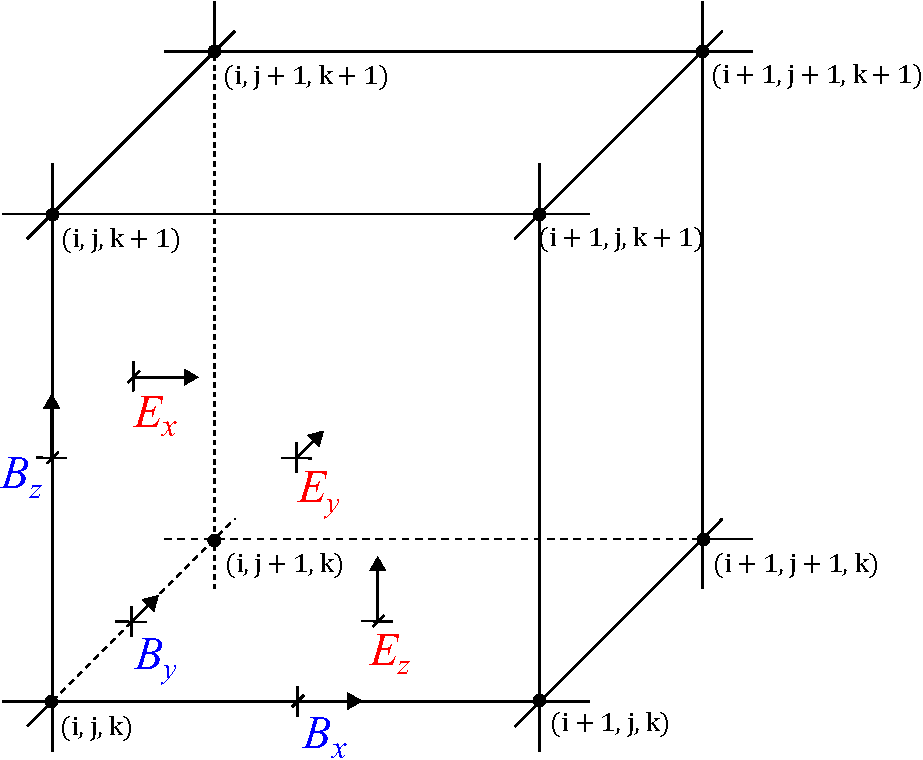
\includegraphics[width=0.35\paperwidth]{./img/yee.pdf}
	\caption[]{\label{fig:yee_lattice} Standard Cartesian Yee cell used in the finite-difference time-domain method. Taken from Ref.~}
\end{figure}

The Maxwell's equations discretized using the leap-frog scheme \cite{Press2007} take the following form,
\begin{equation}\label{eq:discrete_maxwell_1}
	\nabla^{+} \cdot \vec{E}_{ijk}^{\,n} = \frac{\rho_{ijk}^{\,n}}{\varepsilon_0},
\end{equation}
\begin{equation}\label{eq:discrete_maxwell_2}
	\nabla^{-} \cdot \vec{B}_{ijk}^{\,n + 1/2} = 0,
\end{equation}
\begin{equation}\label{eq:discrete_maxwell_3}
	\frac{1}{c^{2}} \frac{\vec{E}_{ijk}^{\,n + 1} - \vec{E}_{ijk}^{\,n}}{\Delta t} = \nabla^{+} \times \vec{B}_{ijk}^{\,n + 1/2} - \mu_{0} \vec{J}_{ijk}^{\,n + 1/2},
\end{equation}
\begin{equation}\label{eq:discrete_maxwell_4}
	\frac{\vec{B}_{ijk}^{\,n + 1/2} - \vec{B}_{ijk}^{\,n - 1/2}}{\Delta t} = -\nabla^{-} \times \vec{E}_{ijk}^{\,n}.
\end{equation}
The operators $ \nabla^{+} $ and $ \nabla^{-} $ used in Eqs.~(\ref{eq:discrete_maxwell_1}) -- (\ref{eq:discrete_maxwell_4}) act on a scalar field $ f_{i j k} $ as follows \cite{Esirkepov2001},
\begin{equation}\label{eq:nabla_plus}
	\nabla^{+} f_{i j k} = \left(\frac{f_{i + 1,\: j,\: k} - f_{i,\: j,\: k}}{\Delta x}, \frac{f_{i,\: j + 1,\: k} - f_{i,\: j,\: k}}{\Delta y}, \frac{f_{i,\: j,\: k + 1} - f_{i,\: j,\: k}}{\Delta z} \right), 
\end{equation}
\begin{equation}\label{eq:nabla_minus}
	\nabla^{-} f_{i j k} = \left(\frac{f_{i,\: j,\: k} - f_{i - 1,\: j,\: k}}{\Delta x}, \frac{f_{i,\: j,\: k} - f_{i,\: j - 1,\: k}}{\Delta y}, \frac{f_{i,\: j,\: k} - f_{i,\: j,\: k - 1}}{\Delta z} \right).
\end{equation}
These operators have the following properties \cite{Esirkepov2001},
\begin{equation}\label{eq:nabla_properties}
	\nabla^{-} \cdot \nabla^{-} \times = \nabla^{+} \cdot \nabla^{+} \times = 0, \qquad \nabla^{-} \cdot \nabla^{+} = \nabla^{+} \cdot \nabla^{-} = \Delta^{\pm},
\end{equation}
where the symbol $ \Delta^{\pm} $ stands for the discrete Laplace operator \cite{Esirkepov2001},
\begin{equation}\label{eq:discrete_laplace}
	\begin{aligned}
	& \quad \quad \quad \Delta^{\pm} f_{i, j, k} = \frac{f_{i - 1, j, k} - 2 f_{i, j, k} + f_{i + 1, j, k}}{\Delta x^{2}} \\[3mm]
	+ & \frac{f_{i, j - 1, k} - 2 f_{i, j, k} + f_{i, j + 1, k}}{\Delta y^{2}} + \frac{f_{i, j, k - 1} - 2 f_{i, j, k} + f_{i, j, k + 1}}{\Delta z^{2}}.
	\end{aligned}
\end{equation}

It is important to realize that, in the three-dimensional case, the system of Eqs.~(\ref{eq:discrete_maxwell_1}) -- (\ref{eq:discrete_maxwell_4}) represents 8 first-order differential equations for 6 unknown vector components. Acting on Eqs.~(\ref{eq:discrete_maxwell_3}) and (\ref{eq:discrete_maxwell_4}) by the operators $ \left(\nabla^{-}\cdot\right) $ and $ \left(\nabla^{+}\cdot\right) $, respectively, one obtains
\begin{equation}\label{eq:discrete_eq_for_B}
	\frac{\nabla^{-} \cdot \vec{B}_{ijk}^{\,n + 1/2} - \nabla^{-} \cdot \vec{B}_{ijk}^{\,n - 1/2}}{\Delta t} = 0,
\end{equation}
\begin{equation}\label{eq:discrete_continuity eq}
	\frac{\rho_{ijk}^{\,n + 1} - \rho_{ijk}^{\,n}}{\Delta t} + \nabla^{+} \cdot \vec{J}_{ijk}^{\,n + 1/2} = 0.
\end{equation}
This means that to get a complete description of the new electric and magnetic fields it is sufficient to calculate only Eqs.~(\ref{eq:discrete_maxwell_3}) and (\ref{eq:discrete_maxwell_4}), while Eqs.~(\ref{eq:discrete_maxwell_1}) and (\ref{eq:discrete_maxwell_2}) can be considered as initial conditions. In such a case, however, the interpolation of charge and current densities on the grid has to satisfy Eq.~(\ref{eq:discrete_continuity eq}).

\subsection{Particle and field weighting}

Let us begin with the deposition of the charge, $ \rho \left( \vec{r}, t \right) $, and current, $ \vec{J} \left( \vec{r}, t \right) $, densities from the quasi-particles to the grid points. According to the kinetic theory, $ \rho \left(\vec{r}, t \right) $ and $ \vec{J} \left( \vec{r}, t \right) $ can be obtained by the following integrals over the momentum space,
\begin{equation}\label{eq:charge_density}
	\rho \left(\vec{r}, t \right) = \sum_s q_s \int f_s \left(\vec{r}, \vec{p}, t \right) \dl \vec{p}, 
\end{equation}
\begin{equation}\label{eq:current_density}
	\vec{J} \left(\vec{r}, t \right) = \sum_s q_s \int f_s \left(\vec{r}, \vec{p}, t \right) \vec{v} \, \dl \vec{p}.
\end{equation}
After discretizing the expressions of Eqs.~(\ref{eq:charge_density}) and (\ref{eq:current_density}) with quasi-particles and using the properties of the shape functions, one gets
\begin{equation}\label{eq:charge_density_discretized}
	\rho_{ijk}^{\,n} = \sum_{p} q_p S^r \left( \vec{r}_{ijk} - \vec{r}_{p}^{\,n} \right),
\end{equation}
\begin{equation}\label{eq:current_density_discretized}
	\vec{J}_{ijk}^{\,n} = \sum_{p} q_p \vec{v}_p^{\,n} S^r \left( \vec{r}_{ijk} - \vec{r}_{p}^{\,n} \right),
\end{equation}
where $ q_p = q_s w_p $. However, the simultaneous use of Eqs.~(\ref{eq:charge_density_discretized}) and (\ref{eq:current_density_discretized}) with arbitrary shape functions always violate Eq.~(\ref{eq:discrete_continuity eq}). To resolve this issue, one would have to calculate Eq.~(\ref{eq:discrete_maxwell_1}) for the correction of the electric field at every simulation time step or use more sophisticated methods that satisfy the continuity equation exactly. These schemes are referred to as the charge conservation methods \cite{Morse1971, Eastwood1991, Villasenor1992, Eastwood1996, Esirkepov2001, Umeda2003}.

%Here we present the method of Ref.~\citenum{bibid} which is valid for arbitrary shape function.




%In order to assign the electric and magnetic fields to the quasi-particle positions, we may s

By analogy to the particle weighting, one may exploit the shape functions to calculate the spatial averages of the electric and magnetic field components,
\begin{equation}\label{key}
	\vec{E}_{p}^{\,n} = \sum_{ijk} \vec{E}_{ijk}^{\,n} S^r \left( \vec{r}_{ijk} - \vec{r}_{p}^{\,n} \right),
\end{equation}
\begin{equation}\label{key}
	\vec{B}_{p}^{\,n} = \sum_{ijk} \vec{B}_{ijk}^{\,n} S^r \left( \vec{r}_{ijk} - \vec{r}_{p}^{\,n} \right).
\end{equation}


%Note that it is recommended to use the same weighting for both, particles and fields, in order to eliminate a self-force and ensure the conservation of momentum \cite{fehske}.

%\subsection{Particle-in-cell algorithm}
%\input{dat/1-0.tex}

%-------------------------------------------------------------------------------

\begin{savequote}[0.45\linewidth]
	\begin{fquote}
		[-- Edward Teller (1908 -- 2003)] The science of today is the technology of tomorrow.
	\end{fquote}
\end{savequote}

\chapter{Author's original results\label{chap:authors_original_results}}
%\input{dat/1-0.tex}

\textsl{In this chapter, the reader can find an overview of the main results achieved within the author's postgraduate studies; in total, we select four papers published in peer-reviewed journals, Refs.~\ref{paper_1} -- \ref{paper_4}, which are fully (or from the most part) based on the author's original work. Below, we provide a brief summary of each selected paper as well as a detailed description of the author's role and contributions. Full texts of all the selected publications are enclosed with permission in Appendix~\ref{chap:selected_publications}.}

\section{On the electromagnetic-electron rings\label{sec:on_the_electromagnetic-electron_rings}}
%\input{dat/1-0.tex}

First, we present the results of research devoted to the coupled electromagnetic and electron rings originating from the interaction of high-power short-pulse laser and underdense plasma, which have been published in Ref.~\ref{paper_1} (the reader can find the full text of the paper in Appendix~\ref{sec:paper_1}). This research has been initiated after the experimental observation of stable and tunable ring-shaped beams of high-energy electrons; the experiment has been carried out by the ELI Beamlines Electron Acceleration Group at the Institute of Plasma Physics and Laser Microfusion in Warsaw, Poland (the reader can find further details in Ref.~\citenum{Grittani2018}). Our preliminary goal was to find out and describe the underlying physical mechanisms which lead to the formation of ring-shaped electron beams in laser plasmas. Although several processes that may result in the electron rings of similar parameters were already identified and presented in literature at that time (see, e.g., Refs.~\citenum{Kaganovich2008, Zhang2012, Pollock2015, Zhao2016, Yang2017, Behm2019, Salehi2021}), none of them seemed to correspond to the particular experimental parameters used in Ref.~\citenum{Grittani2018}.

In general, this work investigates (analytically and using numerical simulations) the propagation of high-power short-pulse laser in a low-density plasma, which is a topic relevant to a number of scientific challenges, such as laser-driven acceleration of charged particles \cite{Tajima1979, Esarey2009, Gonsalves2019}, development of sources of hard electromagnetic radiation \cite{Pirozhkov2012, Bulanov2013}, and nuclear fusion within the framework of the fast ignition concept \cite{Tabak1994}. For most of these applications, it is essential that the laser pulse propagates over extended distances and transmits its energy into the plasma in controlled way without incurring excessive losses. In this context, much of the attention has been focused on the evolution of the radial profile of the laser beam in a fully ionized plasma; it turned out that the process of self-focusing for high-power laser pulses may lead to the formation of the multifilament and, in particular, ring-shaped transverse structures \cite{Mori1988, Cohen1991, Borisov1992, Krushelnick1997, Cattani2001, Kim2002, Naseri2016, Kovalev2019}. We show that these electromagnetic rings can become a source of high-energy ring-shaped electron beams. 

In addition to the applications mentioned above, the understanding of the physical processes that lead to the generation of the electromagnetic and electron ring structures is important due to the following reasons: (i) the electromagnetic rings may carry off a significant fraction of energy from the driver, and thus limit the overall efficiency of applications based on the laser-plasma interaction; (ii) the electron beams accelerated in the wake of the electromagnetic rings may cause a damage to surrounding equipment (e.g., capillaries used for the laser pulse guiding) and become a source of unwanted electromagnetic radiation; and (iii) the knowledge of the origin of the electromagnetic and electron rings could serve as a diagnostics for determining the regimes of laser-plasma interaction.

The first part of the paper presents an analytical model based on geometric optics approximation which qualitatively illustrates the origin and the initial stage of the electromagnetic ring formation. We define the plasma density distribution within the Langmuir wave as well as the Hamiltonian for the photon interaction with the Langmuir wave; the trajectories of photons are then obtained by solving the Hamilton equations. The second part of the paper presents a three-dimensional particle-in-cell simulation, the results of which demonstrate the formation of the electromagnetic as well as electron ring. We discuss the mechanism of formation of the electromagnetic ring and the processes of electron injection into the accelerating phase of the secondary wakefield generated by the electromagnetic ring. Finally, the third part of the paper contains the results of a systematic multi-parametric simulation study for various plasma densities, laser intensities, and laser spot sizes revealing the relationships among the properties of the electromagnetic rings and the parameters of laser and plasma.

The main results of the paper can be summarized as follows. We identify and describe a novel physical mechanism which leads to the formation of ring-shaped electromagnetic-electron structures, where the electromagnetic rings arise from the laser pulse defocusing induced by the excitation of Langmuir waves in underdense plasma, and the ring-shaped electron beams are formed and accelerated subsequently by the secondary toroidal wakefields generated by the electromagnetic rings. We further reveal that the electromagnetic rings are relatively robust nonlinear objects, whose properties can be controlled by tuning the parameters of laser and plasma. Within the studied parameter range, we find that up to $ \approx 70 \ \% $ of the total initial driver pulse energy can be carried off by the electromagnetic rings having the opening angles $ \approx 45 - 115 \ \mathrm{mrad} $. 

Our research published in Ref.~\ref{paper_1} has been promoted by the editors of Physics of Plasmas journal by selecting the article as \q{Featured} and additionally reported by Scilight, which showcases the most interesting research across the physical sciences published in AIP Publishing journals. Furthermore, Fig.~4 from Ref.~\ref{paper_1} has been selected as the cover image of the journal's December issue. Besides Ref.~\ref{paper_1}, a portion of this work has been also published in Ref.~[Valenta SPIE 2021] and presented by the author at \q{SPIE Optics+Optoelectronics 2021,} \q{OPTO2021 Symposium on Photon and Beam Science,} and \q{ELI Summer School 2021,} whereas the latter presentation has been awarded by the \q{Best poster prize.} The author contributed to all the aspects of the research, including the initial formulation of the scientific topic, development of the analytical model, setup and execution of the numerical simulations on computer clusters, and analysis and interpretation of the simulation data. Furthermore, based on the results obtained the author prepared figures, wrote the bulk of the manuscript text, and submitted the manuscript to the journal whereas serving as a corresponding author. Last, the author was communicating with editors and referees concerning the requested revisions of the manuscript until the final publication in the journal.

\section{On the laser-wakefield polarity reversal\label{sec:on_the_laser-wakefield_polarity_reversal}}
%\input{dat/1-0.tex}

Second, we present the results of research devoted to the laser-wakefield acceleration of electrons in the regime of ultrashort pulses and near-critical density plasmas, which have been published in Ref.~\ref{paper_2} (the reader can find the full text of the paper in Appendix~\ref{sec:paper_2}). This research is closely related to the laser-wakefield acceleration of electrons driven by high-repetition-rate ($ \gtrsim \mathrm{kHz} $) laser systems (such as the L1 laser system at ELI Beamlines). 

%The research on laser-wakefield acceleration of electrons has been predominantly oriented on the Joule-class laser systems, which have already demonstrated their capability to produce electron beams at the multi-$ \mathrm{GeV} $ energy scale with a relative energy spread of a few percent \cite{Kim2013, Gonsalves2019}, a few $ \mathrm{fs} $ duration \cite{Tilborg2006, Ohkubo2007, Debus2010, Lundh2011}, and hundreds of $ \mathrm{pC} $ of charge \cite{Li2017, Couperus2017} (although not simultaneously). Recently, however, there has been a growing interest in the laser-wakefield acceleration of electrons driven by high-repetition-rate ($ \gtrsim \mathrm{kHz} $) laser systems since they can significantly improve certain characteristics (e.g., stability, signal-to-noise ratio, and average electron current \cite{Faure2018}) required by a number of practical applications (e.g., ultrafast electron diffraction \cite{Sciaini2011, Miller2014}, $ \mathrm{fs} $ x-ray generation \cite{TaPhuoc2012, Corde2013}, and pulsed radiolysis \cite{Muroya2008}). On the other hand, present-day high-repetition-rate lasers deliver (due to the constraints in technology) pulses with energy of only a few $ \mathrm{mJ} $. This (together with the requirements of the blow-out regime of the laser-wakefield acceleration) implies that, in order to produce high-quality relativistic electron sources, one has to use tightly-focused near-single-cycle pulses and thin near-critical density gas targets \cite{Faure2018, Salehi2019}. Such considerations constitute a great challenge not only from a technical point of view, but also in the sense of the understanding of underlying physical processes (e.g., related to the $ \lambda^{3} $ regime \cite{Mourou2002, Naumova2004}).

The research on laser-wakefield acceleration of electrons has been predominantly oriented on high-energy laser systems. Recently, however, there has been also a growing interest in the laser-wakefield acceleration driven by high-repetition-rate ($ \gtrsim \mathrm{kHz} $) laser systems since they can significantly improve certain characteristics (e.g., stability, signal-to-noise ratio, average electron current \cite{Faure2018}) required by a number of practical applications (e.g., ultrafast electron diffraction \cite{Sciaini2011, Miller2014}, $ \mathrm{fs} $ x-ray generation \cite{TaPhuoc2012, Corde2013}, and pulsed radiolysis \cite{Muroya2008}). On the other hand, present-day high-repetition-rate lasers deliver (due to the constraints in technology) pulses with energy of only a few $ \mathrm{mJ} $. This (together with the requirements of the blow-out regime of the laser-wakefield acceleration) implies that, in order to produce high-quality relativistic electron sources, one has to use tightly-focused near-single-cycle pulses and thin near-critical density gas targets \cite{Faure2018, Salehi2019}. Such considerations constitute a great challenge not only from a technical point of view, but also in the sense of the understanding of underlying physical processes (e.g., related to the $ \lambda^{3} $ regime \cite{Mourou2002, Naumova2004}).

In the first part of the paper we extend the standard model of the wakefield generation by considering the carrier-envelope phase shift of the driving laser pulse. The model shows that wakefield generated by the ultrashort laser pulse contains a long-wavelength modulation of its amplitude. In the second part of the paper we analytically investigate the acceleration of single relativistic electron by the modulated wakefield. We show that the electron energy gain depends on the initial phase of the driver and find the case for which the net energy acquired by the electron over given distance is maximal. Finally, the third part of the paper contains the description of setup and the results of the three-dimensional particle-in-cell simulation on the self-consistent evolution of the ultrashort laser pulse and near-critical density plasma. The simulation results are in qualitative agreement with the analytical model.

The main results of the paper can be summarized as follows. We reveal for the first time (to the best of our knowledge) that the wakefield, being excited by an ultrashort laser pulse in plasma, periodically reverses its polarity. As shown by the analytical model and numerical simulation, the wakefield polarity reversal is caused by dispersion and the corresponding difference between the propagation speed of the carrier and the envelope of the driving laser pulse. Further, we show that the novel phenomenon of the wakefield polarity reversal occurs on spatial scales shorter than the dephasing length and, therefore, significantly affects the energy spectra of accelerated electron beams. In the nonlinear regime, however, there may exist a case for which the polarity reversal length is equal to the dephasing length. In such a case, the dephasing limit is overcome and the electrons are accelerated until the energy of the driver pulse depletes. The discovery of this phenomenon is crucial for better control of the parameters of electron beams accelerated via the laser-wakefield mechanism (e.g., by adjusting the initial phase of the driver or by controlling the phase of the electron injection), particularly in experiments carried out with the present-day high-repetition-rate laser systems.

Besides Ref.~\ref{paper_2}, a portion of this work has been also published in Refs.~[Lazzarini + book, Valenta SPIE 2019, Valenta EPS 2018] and presented by the author at \q{ELI Users' conference 2020,} \q{SPIE Optics+Optoelectronics 2019,} and \q{45$ ^{\mathrm{th}} $ EPS Conference on Plasma Physics,} whereas the latter presentation has been awarded by the \q{Best poster prize.} The author contributed to all the aspects of the research, including the initial formulation of the scientific topic, development of the analytical model, setup and execution of the numerical simulations on computer clusters, and analysis and interpretation of the simulation data. Furthermore, based on the results obtained the author prepared figures and wrote the bulk of the manuscript text, submitted the manuscript to the journal whereas serving as a corresponding author. Last, the author was communicating with editors and referees concerning the requested revisions of the manuscript until the final publication in the journal.

\section{On the recoil effects of relativistic mirrors\label{sec:on_the_recoil_effects_of_relativistic_mirrors}}
%\input{dat/1-0.tex}

Third, we present the results of research devoted to the sources of coherent short-wavelength radiation based on the concept of relativistic flying mirrors in plasma, which have been published in Ref.~\ref{paper_3} (the reader can find the full text of the paper in Appendix~\ref{sec:paper_3}). Maximization of the energy of radiation reflected from the relativistic mirror requires a more intense incident electromagnetic wave. However, sufficiently strong incident light can significantly affect the motion of the relativistic mirror (i.e., its radiation pressure can stop or destroy the mirror). This work investigates (analytically and using numerical simulations) the recoil effects associated with the interaction of relativistic mirrors and strong counter-propagating electromagnetic waves as well as the corresponding changes in the properties of reflected radiation. The considered topic is important for the question of the feasibility of relativistic mirrors for various purposes.

%Relativistic mirrors in plasmas are nowadays actively studied as a unique tool for fundamental research (e.g., light intensification toward the Schwinger limit \cite{Bulanov2003}, investigation of photon–photon and Delbrück scattering \cite{Koga2012, Koga2018}, analog black hole to investigate Hawking radiation and the information loss paradox \cite{Chen2017, Chen2020}) and for many practical applications in diverse fields; depending on whether the configuration is co-propagating or counter-propagating in the laboratory frame of reference, relativistic mirrors might be used either for the acceleration of ions (e.g., for hadron therapy \cite{Bulanov2002}) or for producing coherent high-brightness radiation with wavelengths ranging from x-ray to gamma-ray (e.g., for molecular imaging \cite{Neutze2000} and attosecond spectroscopy \cite{Krausz2009}).

In the first part of the paper we exploit the conservation of momentum and energy before and after the interaction of relativistic flying mirror with counter-propagating electromagnetic wave to develop an analytical model describing the factors of amplification and frequency upshift of the relativistic mirror beyond the approximation of a weak incident electromagnetic wave. Furthermore, we define a threshold for the fluence of the incident electromagnetic wave which characterizes the recoil importance in this interaction. In the second part of the paper, we consider a relativistic flying mirror in the form of strongly nonlinear Langmuir wave and estimate the threshold derived before for this particular case of physical realization of relativistic mirror. Finally, in the third part of the paper we investigate the applicability of our model by one-dimensional particle-in-cell simulations and numerically obtain the properties of interest, such as reflection coefficient of the Langmuir wave and factors of the electric field amplification and the frequency upshift of the incident laser pulse.

The main results of the paper can be summarized as follows. We present an analytical model which shows that if the fluence of the electromagnetic wave incident on the relativistic mirror exceeds a certain threshold, the relativistic mirror undergoes a back reaction significantly affecting its amplification and frequency upshift factors. Further, the numerical simulations reveal that the Langmuir wave driven by a short intense laser pulse in uniform plasma decelerates and, therefore, the reflected radiation has a positive chirp. We find that the electric field amplification factor of the reflected radiation reaches its maximum at the moment of wave-breaking. In addition, our results show that for a given intensity of the source pulse there exists an optimal duration of the source pulse; longer-than-optimal pulses have lower reflected-to-incident energy ratio. Moreover, for a given Langmuir wave excited by the driver pulse there exists an optimal intensity of the source pulse which provides the most intense reflected wave with almost the same frequency upshift factor as in the weak-source approximation.

Besides Ref.~\ref{paper_3}, a portion of this work has been also published in Refs.~[Valenta OSA 2020, Jeong ICXRL 2020] and presented by the author at \q{OSA High-brightness Sources and Light-driven Interactions Congress 2020,} \q{ELI Summer School 2020,} \q{LeCosPA Cosmology and Particle Astrophysics Seminar,} \q{4$ ^{\mathrm{th}} $ Users' Conference of IT4Innovations,} and \q{28$ ^{\mathrm{th}} $ Symposium on Plasma Physics and Technology.} The author contributed to all the aspects of the research, including the initial formulation of the scientific topic, development of the analytical model, setup and execution of the numerical simulations on computer clusters (requiring significant changes to the source code in this case), and analysis and interpretation of the simulation data. Furthermore, based on the results obtained the author prepared figures, wrote the bulk of the manuscript text, and submitted the manuscript to the journal whereas serving as a corresponding author. Last, the author was communicating with editors and referees concerning the requested revisions of the manuscript until the final publication in the journal.


\section{On the relativistic flying forcibly oscillating mirror\label{sec:on_the_relativistic_flying_forcibly_oscillating_mirror}}
%\input{dat/1-0.tex}

The last selected research topic introduces a novel scheme for physical realization of relativistic flying mirrors based on the density singularities in laser plasmas; its results have been published in Ref.~\ref{paper_4} (the reader can find the full text of the paper in Appendix~\ref{sec:paper_4}). In this scheme, the mirror surface is realized by electron density singularities that emerge near the joining area of the wake wave cavity and the bow wave; the mirror moves together with the driving laser pulse and undergoes forced oscillations induced by the driver field. Besides the source pulse base frequency, the spectrum of the reflected light thus contains also its harmonics, all multiplied by a large factor due to the double Doppler effect, which is one of the main advantages of this novel scheme. Furthermore, a counter-propagating laser pulse is incident on the mirror surface at grazing angles, which significantly improves the reflection efficiency.

Apart from the applications mentioned in Sec.~\ref{sec:on_the_recoil_effects_of_relativistic_mirrors}, the scheme described in Ref.~\ref{paper_4} provides an additional tool in laser-plasma diagnostics, helping to analyze the dynamics of nonlinear physical processes in relativistic plasmas. The peculiar spectrum of the reflected radiation in this scheme, using the head-on collision of the driver and source, substantially extends the capabilities for probing relativistic plasma singularities by a transverse source pulse, as suggested in Ref.~\citenum{Esirkepov2020}. Using a weak and short laser pulse as a probe, one can deduce or characterize the parameters of the laser-plasma interaction, including the geometrical properties of the first period of the plasma wave (wake wave cavity and bow wave), driver pulse frequency and magnitude at the location of the mirror, the phase velocity of the wake wave, the electron temperature and momentum distribution at the location of the mirror, etc. 

One of the immediate applications of such a diagnostic is control and tuning of the burst intensification by singularity emitting radiation (BISER) \cite{Pirozhkov2012, Pirozhkov2014, Pirozhkov2017, Sagisaka2020}, which occurs with the same parameters for the driver laser and plasma as required by the described scheme, so that off-axis radiation from the mirror can be observed simultaneously with near- or on-axis BISER. In addition to the fundamental physics concerning intense laser-plasma interactions, plasma diagnostics with the described scheme may help to substantially improve the quality of the laser pulse by revealing what laser parameters are the most critical. Such investigations, in the example of the laser pulse quality effects on the BISER realization, were conducted recently \cite{Pirozhkov2018}. That work revealed some critical parameters of the laser pulse which must be improved to obtain good results and scalings predicted by theory. Last but not least, optical probing of relativistic plasma singularities could reveal a phenomenon similar to the Lampa-Penrose-Terrell effect \cite{Lampa1924, Penrose1959, Terrell1959}, i.e., the image of the constellation of density singularities in plasma would be such as if the singularities were slightly rotated with respect to each other (for closer details see Ref.~\citenum{Esirkepov2020}).

In the first part of the paper we describe the physical mechanisms underlying the formation of the electron density singularities in laser plasmas and propose a novel scheme in which these singularities act as a relativistic mirror. Furthermore, we develop an analytical model in order to predict the base frequency and direction angle of reflected radiation. In the second part of the paper we present a setup and results of three-dimensional and high-resolution two-dimensional particle-in-cell simulations. We demonstrate the feasibility of the novel scheme and analyze the properties of the reflected electromagnetic wave and its spectrum. Finally, in the third part of the paper we investigate the effects of finite temperature on the proposed scheme.

The main results of the paper can be summarized as follows. We propose a novel scheme for physical realization of relativistic mirrors based on the density singularities in laser plasmas - a relativistic flying forcibly oscillating mirror. The proposed scheme uses the electron density singularity at the joining area of the laser wake and bow waves to reflect the counter-propagating source pulse. Since in this regime the surface of the mirror is modulated and oscillates due to the presence of the strong electromagnetic field of the driving laser pulse, it acts as a reflective diffraction grating and generates boosted high-order harmonics of very high brightness. Compared with the boosted high-order harmonics produced by a high-density plasma slab and a thin electron layer \cite{Kulagin2007, Esirkepov2009, Wu2010}, the regime under consideration has the properties of a relativistic flying mirror \cite{Bulanov2003}, relativistic oscillating mirror \cite{Bulanov1994, Naumova2004}, and it inherits the properties of the laser driven oscillating electron spikes \cite{Pirozhkov2014, Pirozhkov2017}. 

Besides Ref.~\ref{paper_4}, a portion of this work has been also published in Refs.~\citenum{Esirkepov2020}[Mu SPIE 2019, Mu Phys. Wave. Phen. 2019] and presented by the author at \q{SPIE Optics \& Photonics International Congress 2019,} \q{KPSI Scientific Seminar,} and \q{2$ ^{\mathrm{nd}} $ Users' Conference of IT4Innovations.} The author contributed mainly to the setup and execution of three-dimensional numerical simulations on computer clusters and subsequent analysis and interpretation of the simulation data. Based on the results obtained the author prepared figures and wrote the bulk of the manuscript text corresponding to the part dealing with the numerical simulations. Last, the author also contributed concerning the requested revisions of the manuscript until the final publication in the journal.





%-------------------------------------------------------------------------------

\begin{savequote}[0.405\linewidth]
	\begin{fquote}
		[-- Voltaire (1694 -- 1778)] The best is the enemy of the good. 
	\end{fquote}
\end{savequote}

\chapter{Conclusion\label{chap:conclusion}}
%\addcontentsline{toc}{chapter}{Conclusion and forthcoming work}
%\input{dat/conclusion.tex}

\section{Summary}

\section{Future research and perspectives}

%Although in the early days the laser was named as \q{a bright solution looking for a problem}, it has since then developed/matured in one of the most important inventions of the last century. It is going to play a even more important role in this century.

%the laser, initially considered as a bright solution looking for a problem, can now properly be indicated as the bright solution of many problems in science and technology

%Applications of lasers have grown spectacularly and now involve many billions of dollars of sale per year

%research with petawatt lasers has been prolific in terms of results with a high potential for applications in several areas,


%\newpage
%\pagestyle{plain}
%\null
%\vfill
%{\bf \noindent Acknowledgments} \\

%I wish express my gratitude to both, my supervisor \klimo and consultant \bulanov for constant support and guidance, as well as for providing invaluable advice and direction.\\

%Access to computing and storage facilities owned by parties and projects contributing to the National Grid Infrastructure MetaCentrum, provided under the programme "Projects of Large Infrastructure for Research, Development, and Innovations" (LM2010005), is greatly appreciated.\\

%Access to the CERIT-SC computing and storage facilities provided under the programme Center CERIT Scientific Cloud, part of the Operational Program Research and Development for Innovations (reg. no. CZ.1.05/3.2.00/08.0144) is greatly  appreciated.\\

%This work was supported by the project ELI: Extreme Light Infrastructure (reg. no. CZ.02.1.01/0.0/0.0/15\_008/0000162) from European Regional Development.\\

%The development of the EPOCH code was funded in part by the UK EPSRC grants EP/G054950/1, EP/G056803/1, EP/G055165/1 and EP/M022463/1.\\
%\begin{flushright}
%\valenta
%\end{flushright}

\newpage

\chapter*{Acknowledgements \markboth{Acknowledgements}{Acknowledgements}}
\addcontentsline{toc}{chapter}{Acknowledgements}

%LeCosPa: Yen-Ling Lee, Mia Wang, Yung-Kun Liu, Yuan Fang, Pisin Chen 
%KPSI: Satoshi Orimo, Timur Esirkepov, James Koga, Alexander Pirozhkov, Masaki Kando, Tetsuya Kawachi
%HIFI: Prokopis Hadjisolomou, Tae-Moon Jeong, David Kolenaty, 
%Office: Elizaveta Pulnova, 

%-------------------------------------------------------------------------------

\newpage
\addcontentsline{toc}{chapter}{Bibliography}
\bibliographystyle{bib/my-apalike}
\bibliography{bib/references}

%-------------------------------------------------------------------------------

\part*{Appendices \markboth{Appendices}{Appendices}}
\addcontentsline{toc}{chapter}{Appendices}

\appendix

\chapter{List of author's publications\label{chap:authors_publications}}

\textsl{Below, the reader can find the full list of publications (as of the day of submission of this dissertation) in peer-reviewed journals, conference proceedings, and as book chapters authored or co-authored by the author during the author's postgraduate studies. The publications are listed in chronological order.}

\section{Publications in peer-reviewed journals\label{sec:peer_reviewed_journals}}

\begin{itemize}
	
	\item Mu, J., Esirkepov, T. Z., \underline{Valenta, P.}, Jeong, T. M., Gu, Y., Koga, J. K., Pirozhkov, A. S., Kando, M., Korn, G., and Bulanov, S. V. (2019). \link{http://dx.doi.org/10.3103/S1541308X19040010}{High-order harmonics from laser irradiated electron density singularity formed at the bow wave in the laser plasma}. \textit{Physics of Wave Phenomena}, \textbf{27}(4):247-256.
	
	\item \underline{Valenta, P.}, Esirkepov, T. Z., Koga, J. K., Pirozhkov, A. S., Kando, M., Kawachi, T., Liu, Y. K., Fang, P., Chen, P., Mu, J., Korn, G., Klimo, O., and Bulanov, S. V. (2020). \link{http://dx.doi.org/10.1063/1.5142084}{Recoil effects on reflection from relativistic mirrors in laser plasmas}., \textit{Physics of Plasmas}, \textbf{27}(3):032109.
	
	\item Esirkepov, T. Z., Mu, J., Gu, Y., Jeong, T. M., \underline{Valenta, P.}, Klimo, O., Koga, J. K., Kando, M., Neely, D., Korn, G., Bulanov, S. V., and Pirozhkov, A. S. (2020). \link{http://dx.doi.org/10.1063/5.0004525}{Optical probing of relativistic plasma singularities}. \textit{Physics of Plasmas}, \textbf{27}(3):052103.
	
	\item Mu, J., Esirkepov, T. Z., \underline{Valenta, P.}, Gu, Y., Jeong, T. M., Pirozhkov, A. S., Koga, J. K., Kando, M., Korn, G., and Bulanov, S. V. (2020). \link{http://dx.doi.org/10.1103/PhysRevE.102.053202}{Relativistic flying forcibly oscillating reflective diffraction grating}. \textit{Physical Review E}, \textbf{102}(5):053202.
	
	\item \underline{Valenta, P.}, Esirkepov, T. Z., Koga, J. K., Nečas, A., Grittani, G. M., Lazzarini, C. M., Klimo, O., Korn, G., and Bulanov, S. V. (2020). \link{http://dx.doi.org/10.1103/PhysRevE.102.053216}{Polarity reversal of wakefields driven by ultrashort pulse laser}. \textit{Physical Review E}, \textbf{102}(5):053216.
	
	\item Hadjisolomou, P., Jeong, T. M., \underline{Valenta, P.}, Korn, G., and Bulanov, S. V. (2021). \link{http://dx.doi.org/10.1103/PhysRevE.104.015203}{Gamma-ray flash generation in irradiating a thin foil target by a single-cycle tightly focused extreme power laser pulse}. \textit{Physical Review E}, \textbf{104}(1):015203.
	
	\item Jeong, T. M., Bulanov, S. V., \underline{Valenta, P.}, Korn, G., Esirkepov, T. Z., Koga, J. K., Pirozhkov, A. S., Kando, M., and Bulanov, S. S. (2021). \link{http://dx.doi.org/10.1103/PhysRevA.104.053533}{Relativistic-flying laser focus by a laser-produced parabolic plasma mirror}. \textit{Physical Review A}, \textbf{104}(6):053533.
	
	\item \underline{Valenta, P.}, Grittani, G. M., Lazzarini, C. M., Klimo, O., and Bulanov, S. V. (2021). \link{http://dx.doi.org/10.1063/5.0065167}{On the electromagnetic-electron rings originating from the interaction of high-power short-pulse laser and underdense plasma}. \textit{Physics of Plasmas}, \textbf{28}(12):122104.
	
	\item Hadjisolomou, P., Jeong, T. M., \underline{Valenta, P.}, Kolenatý, D., Versaci, R., Olšovcová, V., Ridgers, C. P., and Bulanov, S. V. (2021). \link{http://dx.doi.org/}{Gamma-ray flash in the interaction of a tightly focused single-cycle ultraintense laser pulse with a solid target}. \textit{Journal of Plasma Physics}, \textbf{XXX}(X):XXXXXX.
	
\end{itemize}

\section{Publications in conference proceedings\label{sec:conference_proceedings}}

\begin{itemize}
	
	\item Klimo, O., \underline{Valenta, P.}, and Weber, S. (2017). \link{http://ocs.ciemat.es/EPS2017PAP/pdf/P5.225.pdf}{Laser absorption and ion acceleration under tight-focusing conditions}. \textit{44th EPS Conference on Plasma Physics}, P5.225.
	
	\item \underline{Valenta, P.}, Klimo, O., Bulanov, S. V., and Korn, G. (2018). \link{http://ocs.ciemat.es/EPS2018PAP/pdf/P2.2031.pdf}{On high-quality electron beam generated by breaking wake wave in near-critical density plasmas}. \textit{45th EPS Conference on Plasma Physics}, P2.2031. 
	
	\item \underline{Valenta, P.}, Klimo, O., Grittani, G. M., Esirkepov, T. Z., Korn, G., and Bulanov, S. V. (2019). \link{http://dx.doi.org/10.1117/12.2521040}{Wakefield excited by ultrashort laser pulses in near-critical density plasmas}. \textit{Proc. SPIE 11037, Laser Acceleration of Electrons, Protons, and Ions V}, 110370T.
	
	\item Mu, J., Gu, Y., Jeong, T. M., \underline{Valenta, P.}, Klimo, O., Esirkepov, T. Z., Pirozhkov, A. S., Koga, J. K., Kando, M., Korn, G., and Bulanov, S. V. (2019). \link{http://dx.doi.org/10.1117/12.2524653}{High order harmonics generation via laser reflection at electron density peaks}. \textit{Proc. SPIE 11039, Research Using Extreme Light: Entering New Frontiers with Petawatt-Class Lasers IV}, 110390H.
	
	\item Lazzarini, C. M., Goncalves, L. V., Grittani, G. M., Lorenz, S., Nevrkla, M., \underline{Valenta, P.}, Levato, T., Bulanov, S. V., and Korn, G. (2020). \link{http://dx.doi.org/10.1142/S0217751X19430103}{Electron acceleration at ELI Beamlines: towards high-energy and high-repetition-rate accelerators}. \textit{International Journal of Modern Physics A}, \textbf{34}(34):1943010.
	
	\item \underline{Valenta, P.}, Esirkepov, T. Z., Koga, J. K., Pirozhkov, A. S., Kando, M., Kawachi, T., Liu, Y. K., Fang, P., Chen, P., Mu, J., Korn, G., Klimo, O., and Bulanov, S. V. (2020). \link{http://dx.doi.org/10.1364/EUVXRAY.2020.EM1A.5}{Relativistic flying mirrors as a compact source of coherent short-wavelength radiation}. \textit{OSA High-brightness Sources and Light-driven Interactions Congress 2020}, EM1A.5.
	
	\item \underline{Valenta, P.}, Grittani, G. M., Lazzarini, C. M., Klimo, O., and Bulanov, S. V. (2021). \link{http://dx.doi.org/10.1117/12.2589222}{Ring-shaped electron beams from laser-wakefield accelerator}. \textit{Proc. SPIE 11779, Laser Acceleration of Electrons, Protons, and Ions VI}, 1177909.
	
	\item Jeong, T. M., Bulanov, S. V., \underline{Valenta, P.}, Korn, G., Esirkepov, T. Z., Koga, J. K., and Pirozhkov, A. S (2021) \link{http://dx.doi.org/10.1117/12.2592047}{Ultra-strong attosecond laser focus produced by a relativistic-flying parabolic mirror}. \textit{Proc. SPIE 11886, International Conference on X-Ray Lasers 2020}, 118860H.
	
\end{itemize}

\section{Book chapters \label{sec:book_chapters}}

\begin{itemize}
	
	\item Matys, M., Pšikal, J., Danielová, M., \underline{Valenta, P.}, and Bulanov, S. V. (2019). \link{https://www.it4i.cz/cs/file/abd1875ff7d0e6f59799c4f470545516/173/Supercomputing-in-Science-and-Engineering_preview.pdf}{Laser-driven ion acceleration using cryogenic hydrogen targets}. \textit{Supercomputing in Science and Engineering 2017-18}, pp. 149-151.
	
	\item Lazzarini, C. M., Goncalves, L. V., Grittani, G. M., Lorenz, S., Nevrkla, M., \underline{Valenta, P.}, Levato, T., Bulanov, S. V., and Korn, G. (2020) \link{http://dx.doi.org/10.1142/9789811217135_0010}{Electron acceleration at ELI Beamlines: towards high-energy and high-repetition-rate accelerators}. \textit{Beam Acceleration in Crystals and Nanostructures}, pp. 153-170.
	
	\item Matys, M., \underline{Valenta, P.}, Kecová, M., Nishihara, K., Pšikal, J., Esirkepov, T. Z., Koga, J. K., Nečas, A., Grittani, G. M., Lazzarini, C. M., Klimo, O., Korn, G., and Bulanov, S. V. (2021). \link{https://www.it4i.cz/file/be151db89e56452e36511f5410126441/6419/Supercomputing\%20in\%20Science\%20and\%20Engineering\%202019-2020.pdf}{Laser-driven acceleration of charged particles}. \textit{Supercomputing in Science and Engineering 2019-20}, pp. 86-88.
	
\end{itemize}

\chapter{Selected publications\label{chap:selected_publications}}
%\input{dat/appendix_a.tex}

\newpage
\thispagestyle{empty}
\mbox{}

\newpage
\section{On the electromagnetic-electron rings originating from the interaction of high-power short-pulse laser and underdense plasma \label{sec:paper_1}}

The following article is reproduced from Valenta, P., Grittani, G. M., Lazzarini, C. M., Klimo, O., and Bulanov, S. V. (2021). \link{http://dx.doi.org/10.1063/5.0065167}{On the electromagnetic-electron rings originating from the interaction of high-power short-pulse laser and underdense plasma}. \textit{Physics of Plasmas}, \textbf{28}(12):122104, with the permission of AIP Publishing. \\

\noindent Copyright {\copyright} {2021} {American Institute of Physics}.

\newpage
\thispagestyle{empty}
\mbox{}

%\newpage
\includepdf[pages=2-]{misc/paper1.pdf}

%\newpage
%\mbox{}
%\thispagestyle{empty}

\newpage
\section{Polarity reversal of wakefields driven by ultrashort pulse laser \label{sec:paper_2}}

The following article is reproduced from Valenta, P., Esirkepov, T. Z., Koga, J. K., Nečas, A., Grittani, G. M., Lazzarini, C. M., Klimo, O., Korn, G., and Bulanov, S. V. (2020). \link{http://dx.doi.org/10.1103/PhysRevE.102.053216}{Polarity reversal of wakefields driven by ultrashort pulse laser}. \textit{Physical Review E}, \textbf{102}(5):053216, with the permission of APS. \\

\noindent Copyright {\copyright} {2020} {American Physical Society}.

\newpage
\mbox{}
\thispagestyle{empty}

\newpage
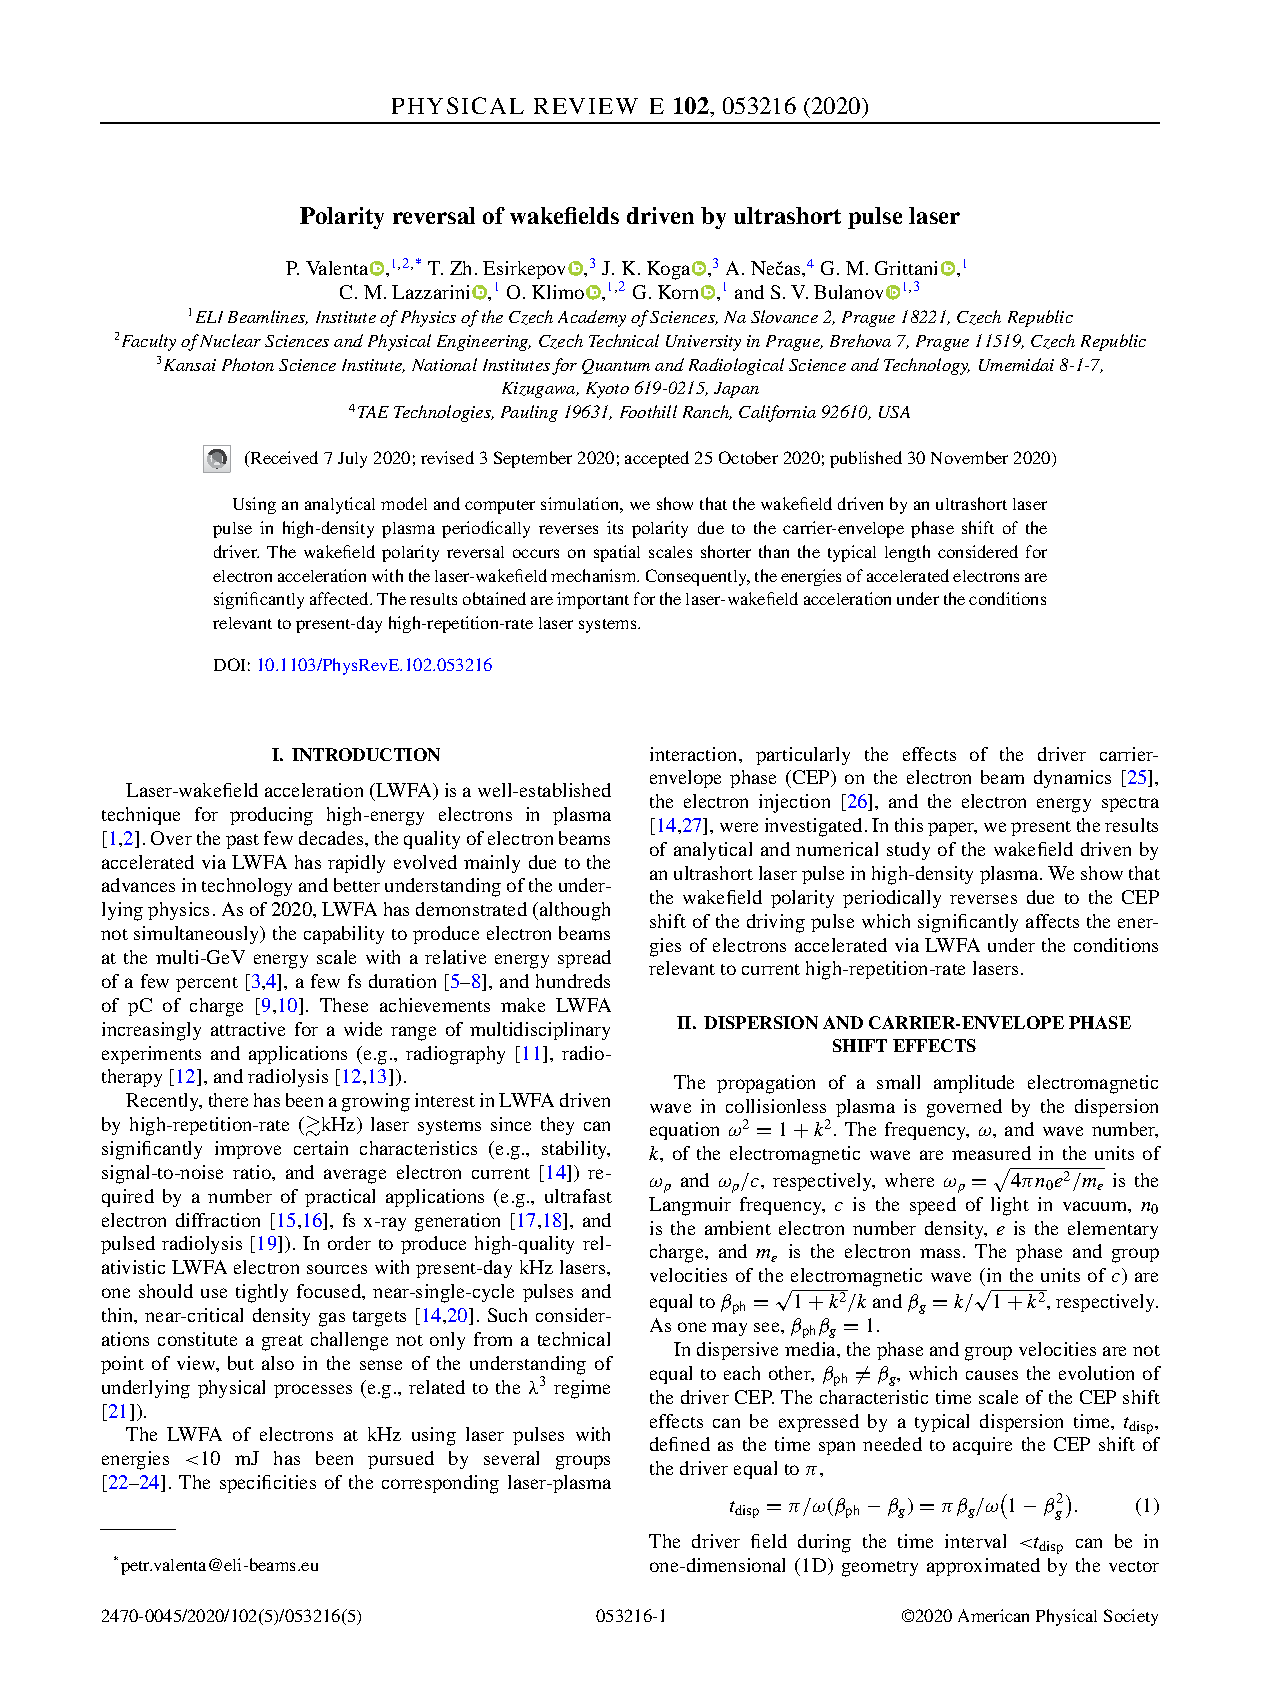
\includepdf[pages=-]{misc/paper2.pdf}

\mbox{}
\thispagestyle{empty}
\newpage

\section{Recoil effects on reflection from relativistic mirrors in laser plasmas \label{sec:paper_3}}

The following article is reproduced from Valenta, P., Esirkepov, T. Z., Koga, J. K., Pirozhkov, A. S., Kando, M., Kawachi, T., Liu, Y. K., Fang, P., Chen, P., Mu, J., Korn, G., Klimo, O., and Bulanov, S. V. (2020). \link{http://dx.doi.org/10.1063/1.5142084}{Recoil effects on reflection from relativistic mirrors in laser plasmas}., \textit{Physics of Plasmas}, \textbf{27}(3):032109, with the permission of AIP Publishing. \\

\noindent Copyright {\copyright} {2020} {American Institute of Physics}.

\newpage
\mbox{}
\thispagestyle{empty}

\newpage
\includepdf[pages=2-]{misc/paper3.pdf}

\section{Relativistic flying forcibly oscillating reflective diffraction grating \label{sec:paper_4}}

The following article is reproduced from Mu, J., Esirkepov, T. Z., Valenta, P., Gu, Y., Jeong, T. M., Pirozhkov, A. S., Koga, J. K., Kando, M., Korn, G., and Bulanov, S. V. (2020). \link{http://dx.doi.org/10.1103/PhysRevE.102.053202}{Relativistic flying forcibly oscillating reflective diffraction grating}. \textit{Physical Review E}, \textbf{102}(5):053202, with the permission of APS. \\

\noindent Copyright {\copyright} {2020} {American Physical Society}.

\newpage
\mbox{}
\thispagestyle{empty}

\newpage
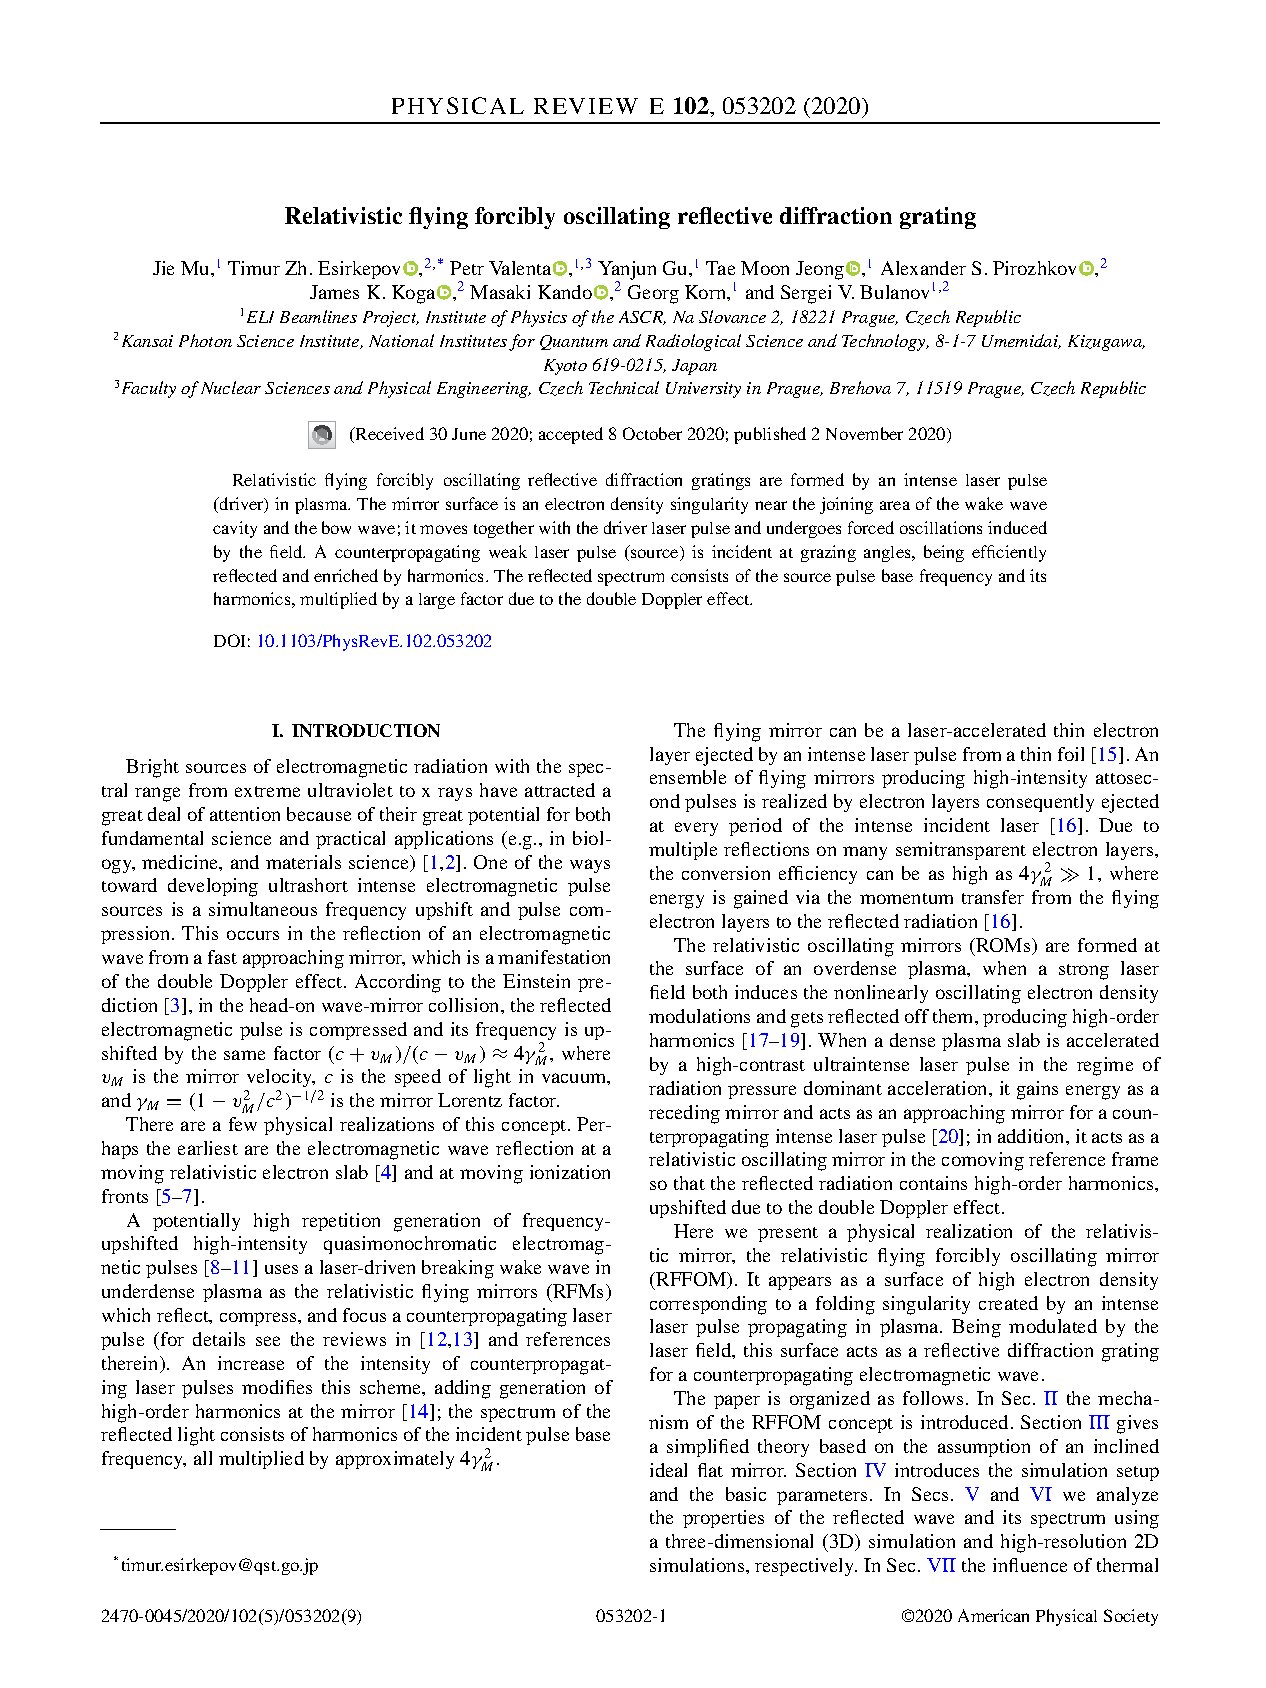
\includepdf[pages=-]{misc/paper4.pdf}

%\chapter{Code listings}
%\input{dat/appendix_b.tex}

%\chapter{CD content}
%\input{dat/appendix_c.tex}

\end{document}